\documentclass[twoside]{book}

% Packages required by doxygen
\usepackage{fixltx2e}
\usepackage{calc}
\usepackage{doxygen}
\usepackage{graphicx}
\usepackage[utf8]{inputenc}
\usepackage{makeidx}
\usepackage{multicol}
\usepackage{multirow}
\PassOptionsToPackage{warn}{textcomp}
\usepackage{textcomp}
\usepackage[nointegrals]{wasysym}
\usepackage[table]{xcolor}

% NLS support packages
\usepackage{hfont}

% Font selection
\usepackage[T1]{fontenc}
\usepackage{mathptmx}
\usepackage[scaled=.90]{helvet}
\usepackage{courier}
\usepackage{amssymb}
\usepackage{sectsty}
\renewcommand{\familydefault}{\sfdefault}
\allsectionsfont{%
  \fontseries{bc}\selectfont%
  \color{darkgray}%
}
\renewcommand{\DoxyLabelFont}{%
  \fontseries{bc}\selectfont%
  \color{darkgray}%
}
\newcommand{\+}{\discretionary{\mbox{\scriptsize$\hookleftarrow$}}{}{}}

% Page & text layout
\usepackage{geometry}
\geometry{%
  a4paper,%
  top=2.5cm,%
  bottom=2.5cm,%
  left=2.5cm,%
  right=2.5cm%
}
\tolerance=750
\hfuzz=15pt
\hbadness=750
\setlength{\emergencystretch}{15pt}
\setlength{\parindent}{0cm}
\setlength{\parskip}{0.2cm}
\makeatletter
\renewcommand{\paragraph}{%
  \@startsection{paragraph}{4}{0ex}{-1.0ex}{1.0ex}{%
    \normalfont\normalsize\bfseries\SS@parafont%
  }%
}
\renewcommand{\subparagraph}{%
  \@startsection{subparagraph}{5}{0ex}{-1.0ex}{1.0ex}{%
    \normalfont\normalsize\bfseries\SS@subparafont%
  }%
}
\makeatother

% Headers & footers
\usepackage{fancyhdr}
\pagestyle{fancyplain}
\fancyhead[LE]{\fancyplain{}{\bfseries\thepage}}
\fancyhead[CE]{\fancyplain{}{}}
\fancyhead[RE]{\fancyplain{}{\bfseries\leftmark}}
\fancyhead[LO]{\fancyplain{}{\bfseries\rightmark}}
\fancyhead[CO]{\fancyplain{}{}}
\fancyhead[RO]{\fancyplain{}{\bfseries\thepage}}
\fancyfoot[LE]{\fancyplain{}{}}
\fancyfoot[CE]{\fancyplain{}{}}
\fancyfoot[RE]{\fancyplain{}{\bfseries\scriptsize 생성시간 \+: 토 11월 22 2014 05\+:06\+:00, 프로젝트명 \+: L\+R\+U cache simulator, 생성자 \+:  Doxygen }}
\fancyfoot[LO]{\fancyplain{}{\bfseries\scriptsize 생성시간 \+: 토 11월 22 2014 05\+:06\+:00, 프로젝트명 \+: L\+R\+U cache simulator, 생성자 \+:  Doxygen }}
\fancyfoot[CO]{\fancyplain{}{}}
\fancyfoot[RO]{\fancyplain{}{}}
\renewcommand{\footrulewidth}{0.4pt}
\renewcommand{\chaptermark}[1]{%
  \markboth{#1}{}%
}
\renewcommand{\sectionmark}[1]{%
  \markright{\thesection\ #1}%
}

% Indices & bibliography
\usepackage{natbib}
\usepackage[titles]{tocloft}
\setcounter{tocdepth}{3}
\setcounter{secnumdepth}{5}
\makeindex

% Hyperlinks (required, but should be loaded last)
\usepackage{ifpdf}
\ifpdf
  \usepackage[pdftex,pagebackref=true]{hyperref}
\else
  \usepackage[ps2pdf,pagebackref=true]{hyperref}
\fi
\hypersetup{%
  colorlinks=true,%
  linkcolor=blue,%
  citecolor=blue,%
  unicode%
}

% Custom commands
\newcommand{\clearemptydoublepage}{%
  \newpage{\pagestyle{empty}\cleardoublepage}%
}


%===== C O N T E N T S =====

\begin{document}

% Titlepage & ToC
\hypersetup{pageanchor=false,
             bookmarks=true,
             bookmarksnumbered=true,
             pdfencoding=unicode
            }
\pagenumbering{roman}
\begin{titlepage}
\vspace*{7cm}
\begin{center}%
{\Large L\+R\+U cache simulator \\[1ex]\large 0.\+9.\+0 }\\
\vspace*{1cm}
{\large 다음에 의해 생성됨 \+:  Doxygen 1.8.8}\\
\vspace*{0.5cm}
{\small 토 11월 22 2014 05:06:00}\\
\end{center}
\end{titlepage}
\clearemptydoublepage
\tableofcontents
\clearemptydoublepage
\pagenumbering{arabic}
\hypersetup{pageanchor=true}

%--- Begin generated contents ---
\chapter{클래스 색인}
\section{클래스 목록}
다음은 클래스, 구조체, 공용체 그리고 인터페이스들입니다. (간략한 설명만을 보여줍니다) \+:\begin{DoxyCompactList}
\item\contentsline{section}{\hyperlink{structanalysis__arg}{analysis\+\_\+arg} }{\pageref{structanalysis__arg}}{}
\item\contentsline{section}{\hyperlink{structcache__line}{cache\+\_\+line} }{\pageref{structcache__line}}{}
\item\contentsline{section}{\hyperlink{structcache__mem}{cache\+\_\+mem} }{\pageref{structcache__mem}}{}
\item\contentsline{section}{\hyperlink{structcode__info}{code\+\_\+info} }{\pageref{structcode__info}}{}
\item\contentsline{section}{\hyperlink{structdk__tnode}{dk\+\_\+tnode} }{\pageref{structdk__tnode}}{}
\item\contentsline{section}{\hyperlink{structdk__tree}{dk\+\_\+tree} }{\pageref{structdk__tree}}{}
\item\contentsline{section}{\hyperlink{structfile__info}{file\+\_\+info} }{\pageref{structfile__info}}{}
\item\contentsline{section}{\hyperlink{structhash__row}{hash\+\_\+row} }{\pageref{structhash__row}}{}
\item\contentsline{section}{\hyperlink{structhash__table}{hash\+\_\+table} }{\pageref{structhash__table}}{}
\item\contentsline{section}{\hyperlink{structlist__head}{list\+\_\+head} }{\pageref{structlist__head}}{}
\item\contentsline{section}{\hyperlink{structworkload}{workload} }{\pageref{structworkload}}{}
\end{DoxyCompactList}

\chapter{파일 색인}
\section{File List}
Here is a list of all files with brief descriptions\+:\begin{DoxyCompactList}
\item\contentsline{section}{\hyperlink{main_8c}{main.\+c} }{\pageref{main_8c}}{}
\end{DoxyCompactList}

\chapter{클래스 문서화}
\hypertarget{structanalysis__arg}{\section{analysis\+\_\+arg 구조체 참조}
\label{structanalysis__arg}\index{analysis\+\_\+arg@{analysis\+\_\+arg}}
}


{\ttfamily \#include $<$code\+\_\+analyze.\+h$>$}



analysis\+\_\+arg에 대한 협력 다이어그램\+:
\nopagebreak
\begin{figure}[H]
\begin{center}
\leavevmode
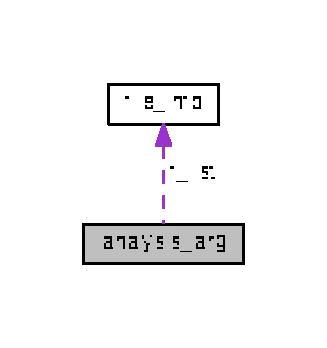
\includegraphics[width=157pt]{structanalysis__arg__coll__graph}
\end{center}
\end{figure}
\subsection*{Public 속성}
\begin{DoxyCompactItemize}
\item 
char $\ast$ \hyperlink{structanalysis__arg_ae4dc80fc7340c819c3315324b1c24511}{f\+\_\+name}
\item 
struct \hyperlink{structfile__info}{file\+\_\+info} $\ast$ \hyperlink{structanalysis__arg_a06dce9c50b6212f9fd620d149adc5734}{f\+\_\+list}
\item 
int \hyperlink{structanalysis__arg_af120d208cb66f64281db9ccd6f2f6afc}{num}
\item 
pthread\+\_\+mutex\+\_\+t $\ast$ \hyperlink{structanalysis__arg_a5af66e583b346de25aee6ab4acaa91a7}{mutex}
\end{DoxyCompactItemize}


\subsection{멤버 데이타 문서화}
\hypertarget{structanalysis__arg_a06dce9c50b6212f9fd620d149adc5734}{\index{analysis\+\_\+arg@{analysis\+\_\+arg}!f\+\_\+list@{f\+\_\+list}}
\index{f\+\_\+list@{f\+\_\+list}!analysis\+\_\+arg@{analysis\+\_\+arg}}
\subsubsection[{f\+\_\+list}]{\setlength{\rightskip}{0pt plus 5cm}struct {\bf file\+\_\+info}$\ast$ analysis\+\_\+arg\+::f\+\_\+list}}\label{structanalysis__arg_a06dce9c50b6212f9fd620d149adc5734}
\hypertarget{structanalysis__arg_ae4dc80fc7340c819c3315324b1c24511}{\index{analysis\+\_\+arg@{analysis\+\_\+arg}!f\+\_\+name@{f\+\_\+name}}
\index{f\+\_\+name@{f\+\_\+name}!analysis\+\_\+arg@{analysis\+\_\+arg}}
\subsubsection[{f\+\_\+name}]{\setlength{\rightskip}{0pt plus 5cm}char$\ast$ analysis\+\_\+arg\+::f\+\_\+name}}\label{structanalysis__arg_ae4dc80fc7340c819c3315324b1c24511}
\hypertarget{structanalysis__arg_a5af66e583b346de25aee6ab4acaa91a7}{\index{analysis\+\_\+arg@{analysis\+\_\+arg}!mutex@{mutex}}
\index{mutex@{mutex}!analysis\+\_\+arg@{analysis\+\_\+arg}}
\subsubsection[{mutex}]{\setlength{\rightskip}{0pt plus 5cm}pthread\+\_\+mutex\+\_\+t$\ast$ analysis\+\_\+arg\+::mutex}}\label{structanalysis__arg_a5af66e583b346de25aee6ab4acaa91a7}
\hypertarget{structanalysis__arg_af120d208cb66f64281db9ccd6f2f6afc}{\index{analysis\+\_\+arg@{analysis\+\_\+arg}!num@{num}}
\index{num@{num}!analysis\+\_\+arg@{analysis\+\_\+arg}}
\subsubsection[{num}]{\setlength{\rightskip}{0pt plus 5cm}int analysis\+\_\+arg\+::num}}\label{structanalysis__arg_af120d208cb66f64281db9ccd6f2f6afc}


이 구조체에 대한 문서화 페이지는 다음의 파일로부터 생성되었습니다.\+:\begin{DoxyCompactItemize}
\item 
dkh/\hyperlink{code__analyze_8h}{code\+\_\+analyze.\+h}\end{DoxyCompactItemize}

\hypertarget{structcache__line}{\section{cache\+\_\+line Struct Reference}
\label{structcache__line}\index{cache\+\_\+line@{cache\+\_\+line}}
}


{\ttfamily \#include $<$lru.\+h$>$}



Collaboration diagram for cache\+\_\+line\+:
\subsection*{Public Attributes}
\begin{DoxyCompactItemize}
\item 
long \hyperlink{structcache__line_a22870a00436e7425597606393d81eb2c}{line}
\item 
struct \hyperlink{structlist__head}{list\+\_\+head} \hyperlink{structcache__line_af231d538713478b74fc7811adc00545b}{head}
\end{DoxyCompactItemize}


\subsection{Member Data Documentation}
\hypertarget{structcache__line_af231d538713478b74fc7811adc00545b}{\index{cache\+\_\+line@{cache\+\_\+line}!head@{head}}
\index{head@{head}!cache\+\_\+line@{cache\+\_\+line}}
\subsubsection[{head}]{\setlength{\rightskip}{0pt plus 5cm}struct {\bf list\+\_\+head} cache\+\_\+line\+::head}}\label{structcache__line_af231d538713478b74fc7811adc00545b}
\hypertarget{structcache__line_a22870a00436e7425597606393d81eb2c}{\index{cache\+\_\+line@{cache\+\_\+line}!line@{line}}
\index{line@{line}!cache\+\_\+line@{cache\+\_\+line}}
\subsubsection[{line}]{\setlength{\rightskip}{0pt plus 5cm}long cache\+\_\+line\+::line}}\label{structcache__line_a22870a00436e7425597606393d81eb2c}


The documentation for this struct was generated from the following file\+:\begin{DoxyCompactItemize}
\item 
dkh/\hyperlink{lru_8h}{lru.\+h}\end{DoxyCompactItemize}

\hypertarget{structcache__mem}{\section{cache\+\_\+mem 구조체 참조}
\label{structcache__mem}\index{cache\+\_\+mem@{cache\+\_\+mem}}
}


{\ttfamily \#include $<$lru.\+h$>$}



cache\+\_\+mem에 대한 협력 다이어그램\+:
\nopagebreak
\begin{figure}[H]
\begin{center}
\leavevmode
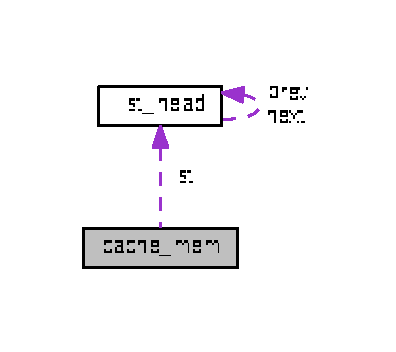
\includegraphics[width=190pt]{structcache__mem__coll__graph}
\end{center}
\end{figure}
\subsection*{Public 속성}
\begin{DoxyCompactItemize}
\item 
struct \hyperlink{structlist__head}{list\+\_\+head} $\ast$ \hyperlink{structcache__mem_a785dde86afb87f8825779f50e29d6bd7}{list}
\item 
long \hyperlink{structcache__mem_a58c6a91c40d59398a3ed18daccc448fc}{size}
\item 
long \hyperlink{structcache__mem_aca41dfab3073387e6c6063457a17f616}{max}
\item 
long \hyperlink{structcache__mem_af64061b621392a1872f5cb92dde7dc7c}{read}
\item 
long \hyperlink{structcache__mem_adb5a0315176779908235c7ed3e41ec57}{write}
\item 
long \hyperlink{structcache__mem_a2b8742701cf4beaff0639d36d52209d9}{hit}
\end{DoxyCompactItemize}


\subsection{멤버 데이타 문서화}
\hypertarget{structcache__mem_a2b8742701cf4beaff0639d36d52209d9}{\index{cache\+\_\+mem@{cache\+\_\+mem}!hit@{hit}}
\index{hit@{hit}!cache\+\_\+mem@{cache\+\_\+mem}}
\subsubsection[{hit}]{\setlength{\rightskip}{0pt plus 5cm}long cache\+\_\+mem\+::hit}}\label{structcache__mem_a2b8742701cf4beaff0639d36d52209d9}
\hypertarget{structcache__mem_a785dde86afb87f8825779f50e29d6bd7}{\index{cache\+\_\+mem@{cache\+\_\+mem}!list@{list}}
\index{list@{list}!cache\+\_\+mem@{cache\+\_\+mem}}
\subsubsection[{list}]{\setlength{\rightskip}{0pt plus 5cm}struct {\bf list\+\_\+head}$\ast$ cache\+\_\+mem\+::list}}\label{structcache__mem_a785dde86afb87f8825779f50e29d6bd7}
\hypertarget{structcache__mem_aca41dfab3073387e6c6063457a17f616}{\index{cache\+\_\+mem@{cache\+\_\+mem}!max@{max}}
\index{max@{max}!cache\+\_\+mem@{cache\+\_\+mem}}
\subsubsection[{max}]{\setlength{\rightskip}{0pt plus 5cm}long cache\+\_\+mem\+::max}}\label{structcache__mem_aca41dfab3073387e6c6063457a17f616}
\hypertarget{structcache__mem_af64061b621392a1872f5cb92dde7dc7c}{\index{cache\+\_\+mem@{cache\+\_\+mem}!read@{read}}
\index{read@{read}!cache\+\_\+mem@{cache\+\_\+mem}}
\subsubsection[{read}]{\setlength{\rightskip}{0pt plus 5cm}long cache\+\_\+mem\+::read}}\label{structcache__mem_af64061b621392a1872f5cb92dde7dc7c}
\hypertarget{structcache__mem_a58c6a91c40d59398a3ed18daccc448fc}{\index{cache\+\_\+mem@{cache\+\_\+mem}!size@{size}}
\index{size@{size}!cache\+\_\+mem@{cache\+\_\+mem}}
\subsubsection[{size}]{\setlength{\rightskip}{0pt plus 5cm}long cache\+\_\+mem\+::size}}\label{structcache__mem_a58c6a91c40d59398a3ed18daccc448fc}
\hypertarget{structcache__mem_adb5a0315176779908235c7ed3e41ec57}{\index{cache\+\_\+mem@{cache\+\_\+mem}!write@{write}}
\index{write@{write}!cache\+\_\+mem@{cache\+\_\+mem}}
\subsubsection[{write}]{\setlength{\rightskip}{0pt plus 5cm}long cache\+\_\+mem\+::write}}\label{structcache__mem_adb5a0315176779908235c7ed3e41ec57}


이 구조체에 대한 문서화 페이지는 다음의 파일로부터 생성되었습니다.\+:\begin{DoxyCompactItemize}
\item 
dkh/\hyperlink{lru_8h}{lru.\+h}\end{DoxyCompactItemize}

\hypertarget{structcode__info}{\section{code\+\_\+info Struct Reference}
\label{structcode__info}\index{code\+\_\+info@{code\+\_\+info}}
}


{\ttfamily \#include $<$code\+\_\+analyze.\+h$>$}

\subsection*{Public Attributes}
\begin{DoxyCompactItemize}
\item 
char $\ast$ \hyperlink{structcode__info_ab511aa50afcbcfc1bb2fa4b4a6012e6b}{name}
\item 
int \hyperlink{structcode__info_ad2648840a6e7ba7c9c02ec444a3adac2}{line}
\item 
int \hyperlink{structcode__info_a06f6c405ef67eb10711dc4fbc90e52c2}{b\+\_\+l}
\item 
int \hyperlink{structcode__info_a4dc2ea78ef6f9f8f1fea89fd42f7bf18}{b\+\_\+m}
\item 
int \hyperlink{structcode__info_a881e5abdce42a2de03dd079ee7ae3304}{b\+\_\+s}
\item 
int \hyperlink{structcode__info_a091007c87af472a025bc06633218e344}{f\+\_\+count}
\item 
int \hyperlink{structcode__info_a8a9fc76d0701714e834a52a66b82156e}{f\+\_\+maxline}
\item 
int \hyperlink{structcode__info_ac0a3b579d41a998a2aec410925032aa7}{f\+\_\+minline}
\end{DoxyCompactItemize}


\subsection{Member Data Documentation}
\hypertarget{structcode__info_a06f6c405ef67eb10711dc4fbc90e52c2}{\index{code\+\_\+info@{code\+\_\+info}!b\+\_\+l@{b\+\_\+l}}
\index{b\+\_\+l@{b\+\_\+l}!code\+\_\+info@{code\+\_\+info}}
\subsubsection[{b\+\_\+l}]{\setlength{\rightskip}{0pt plus 5cm}int code\+\_\+info\+::b\+\_\+l}}\label{structcode__info_a06f6c405ef67eb10711dc4fbc90e52c2}
\hypertarget{structcode__info_a4dc2ea78ef6f9f8f1fea89fd42f7bf18}{\index{code\+\_\+info@{code\+\_\+info}!b\+\_\+m@{b\+\_\+m}}
\index{b\+\_\+m@{b\+\_\+m}!code\+\_\+info@{code\+\_\+info}}
\subsubsection[{b\+\_\+m}]{\setlength{\rightskip}{0pt plus 5cm}int code\+\_\+info\+::b\+\_\+m}}\label{structcode__info_a4dc2ea78ef6f9f8f1fea89fd42f7bf18}
\hypertarget{structcode__info_a881e5abdce42a2de03dd079ee7ae3304}{\index{code\+\_\+info@{code\+\_\+info}!b\+\_\+s@{b\+\_\+s}}
\index{b\+\_\+s@{b\+\_\+s}!code\+\_\+info@{code\+\_\+info}}
\subsubsection[{b\+\_\+s}]{\setlength{\rightskip}{0pt plus 5cm}int code\+\_\+info\+::b\+\_\+s}}\label{structcode__info_a881e5abdce42a2de03dd079ee7ae3304}
\hypertarget{structcode__info_a091007c87af472a025bc06633218e344}{\index{code\+\_\+info@{code\+\_\+info}!f\+\_\+count@{f\+\_\+count}}
\index{f\+\_\+count@{f\+\_\+count}!code\+\_\+info@{code\+\_\+info}}
\subsubsection[{f\+\_\+count}]{\setlength{\rightskip}{0pt plus 5cm}int code\+\_\+info\+::f\+\_\+count}}\label{structcode__info_a091007c87af472a025bc06633218e344}
\hypertarget{structcode__info_a8a9fc76d0701714e834a52a66b82156e}{\index{code\+\_\+info@{code\+\_\+info}!f\+\_\+maxline@{f\+\_\+maxline}}
\index{f\+\_\+maxline@{f\+\_\+maxline}!code\+\_\+info@{code\+\_\+info}}
\subsubsection[{f\+\_\+maxline}]{\setlength{\rightskip}{0pt plus 5cm}int code\+\_\+info\+::f\+\_\+maxline}}\label{structcode__info_a8a9fc76d0701714e834a52a66b82156e}
\hypertarget{structcode__info_ac0a3b579d41a998a2aec410925032aa7}{\index{code\+\_\+info@{code\+\_\+info}!f\+\_\+minline@{f\+\_\+minline}}
\index{f\+\_\+minline@{f\+\_\+minline}!code\+\_\+info@{code\+\_\+info}}
\subsubsection[{f\+\_\+minline}]{\setlength{\rightskip}{0pt plus 5cm}int code\+\_\+info\+::f\+\_\+minline}}\label{structcode__info_ac0a3b579d41a998a2aec410925032aa7}
\hypertarget{structcode__info_ad2648840a6e7ba7c9c02ec444a3adac2}{\index{code\+\_\+info@{code\+\_\+info}!line@{line}}
\index{line@{line}!code\+\_\+info@{code\+\_\+info}}
\subsubsection[{line}]{\setlength{\rightskip}{0pt plus 5cm}int code\+\_\+info\+::line}}\label{structcode__info_ad2648840a6e7ba7c9c02ec444a3adac2}
\hypertarget{structcode__info_ab511aa50afcbcfc1bb2fa4b4a6012e6b}{\index{code\+\_\+info@{code\+\_\+info}!name@{name}}
\index{name@{name}!code\+\_\+info@{code\+\_\+info}}
\subsubsection[{name}]{\setlength{\rightskip}{0pt plus 5cm}char$\ast$ code\+\_\+info\+::name}}\label{structcode__info_ab511aa50afcbcfc1bb2fa4b4a6012e6b}


The documentation for this struct was generated from the following file\+:\begin{DoxyCompactItemize}
\item 
dkh/\hyperlink{code__analyze_8h}{code\+\_\+analyze.\+h}\end{DoxyCompactItemize}

\hypertarget{structdk__tnode}{\section{dk\+\_\+tnode Struct Reference}
\label{structdk__tnode}\index{dk\+\_\+tnode@{dk\+\_\+tnode}}
}


{\ttfamily \#include $<$dk\+\_\+tree.\+h$>$}



Collaboration diagram for dk\+\_\+tnode\+:
\subsection*{Public Attributes}
\begin{DoxyCompactItemize}
\item 
void $\ast$ \hyperlink{structdk__tnode_a4d8427a1419ca15308105dae0621c2bf}{c}
\item 
struct \hyperlink{structdk__tnode}{dk\+\_\+tnode} $\ast$ \hyperlink{structdk__tnode_a3a3fdb7d00634c393fad557eb15f0166}{p}
\item 
struct \hyperlink{structdk__tnode}{dk\+\_\+tnode} $\ast$ \hyperlink{structdk__tnode_a13392f297542ba6ec06da4e389ef3d7f}{r}
\item 
struct \hyperlink{structdk__tnode}{dk\+\_\+tnode} $\ast$ \hyperlink{structdk__tnode_acf718a20eaecd8c363ef2f70742013a5}{l}
\end{DoxyCompactItemize}


\subsection{Member Data Documentation}
\hypertarget{structdk__tnode_a4d8427a1419ca15308105dae0621c2bf}{\index{dk\+\_\+tnode@{dk\+\_\+tnode}!c@{c}}
\index{c@{c}!dk\+\_\+tnode@{dk\+\_\+tnode}}
\subsubsection[{c}]{\setlength{\rightskip}{0pt plus 5cm}void$\ast$ dk\+\_\+tnode\+::c}}\label{structdk__tnode_a4d8427a1419ca15308105dae0621c2bf}
\hypertarget{structdk__tnode_acf718a20eaecd8c363ef2f70742013a5}{\index{dk\+\_\+tnode@{dk\+\_\+tnode}!l@{l}}
\index{l@{l}!dk\+\_\+tnode@{dk\+\_\+tnode}}
\subsubsection[{l}]{\setlength{\rightskip}{0pt plus 5cm}struct {\bf dk\+\_\+tnode}$\ast$ dk\+\_\+tnode\+::l}}\label{structdk__tnode_acf718a20eaecd8c363ef2f70742013a5}
\hypertarget{structdk__tnode_a3a3fdb7d00634c393fad557eb15f0166}{\index{dk\+\_\+tnode@{dk\+\_\+tnode}!p@{p}}
\index{p@{p}!dk\+\_\+tnode@{dk\+\_\+tnode}}
\subsubsection[{p}]{\setlength{\rightskip}{0pt plus 5cm}struct {\bf dk\+\_\+tnode}$\ast$ dk\+\_\+tnode\+::p}}\label{structdk__tnode_a3a3fdb7d00634c393fad557eb15f0166}
\hypertarget{structdk__tnode_a13392f297542ba6ec06da4e389ef3d7f}{\index{dk\+\_\+tnode@{dk\+\_\+tnode}!r@{r}}
\index{r@{r}!dk\+\_\+tnode@{dk\+\_\+tnode}}
\subsubsection[{r}]{\setlength{\rightskip}{0pt plus 5cm}struct {\bf dk\+\_\+tnode}$\ast$ dk\+\_\+tnode\+::r}}\label{structdk__tnode_a13392f297542ba6ec06da4e389ef3d7f}


The documentation for this struct was generated from the following file\+:\begin{DoxyCompactItemize}
\item 
dkh/\hyperlink{dk__tree_8h}{dk\+\_\+tree.\+h}\end{DoxyCompactItemize}

\hypertarget{structdk__tree}{\section{dk\+\_\+tree 구조체 참조}
\label{structdk__tree}\index{dk\+\_\+tree@{dk\+\_\+tree}}
}


{\ttfamily \#include $<$dk\+\_\+tree.\+h$>$}



dk\+\_\+tree에 대한 협력 다이어그램\+:
\nopagebreak
\begin{figure}[H]
\begin{center}
\leavevmode
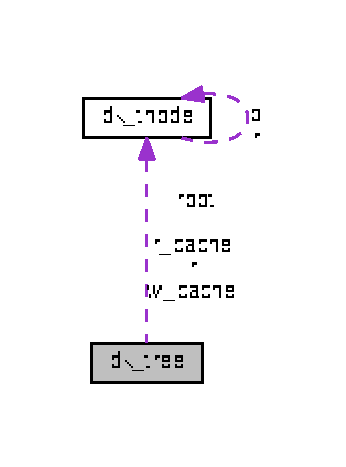
\includegraphics[width=166pt]{structdk__tree__coll__graph}
\end{center}
\end{figure}
\subsection*{Public 속성}
\begin{DoxyCompactItemize}
\item 
int \hyperlink{structdk__tree_af79ecba1677f82486893accb0859a696}{count}
\item 
struct \hyperlink{structdk__tnode}{dk\+\_\+tnode} $\ast$ \hyperlink{structdk__tree_a6a5c48e2ff2494e10aafd1d0bc9d5992}{root}
\item 
struct \hyperlink{structdk__tnode}{dk\+\_\+tnode} $\ast$ \hyperlink{structdk__tree_a5d989a0efeadbc970750f1ac8ad4018e}{r}
\item 
struct \hyperlink{structdk__tnode}{dk\+\_\+tnode} $\ast$ \hyperlink{structdk__tree_a47101f1a0d29f4be791707a4b4b6477e}{l}
\item 
struct \hyperlink{structdk__tnode}{dk\+\_\+tnode} $\ast$ \hyperlink{structdk__tree_ae1a363a68dda726e3010e6766057dbbe}{r\+\_\+cache}
\item 
struct \hyperlink{structdk__tnode}{dk\+\_\+tnode} $\ast$ \hyperlink{structdk__tree_ab968d09f4098a59419b509bce61debcb}{w\+\_\+cache}
\end{DoxyCompactItemize}


\subsection{멤버 데이타 문서화}
\hypertarget{structdk__tree_af79ecba1677f82486893accb0859a696}{\index{dk\+\_\+tree@{dk\+\_\+tree}!count@{count}}
\index{count@{count}!dk\+\_\+tree@{dk\+\_\+tree}}
\subsubsection[{count}]{\setlength{\rightskip}{0pt plus 5cm}int dk\+\_\+tree\+::count}}\label{structdk__tree_af79ecba1677f82486893accb0859a696}
\hypertarget{structdk__tree_a47101f1a0d29f4be791707a4b4b6477e}{\index{dk\+\_\+tree@{dk\+\_\+tree}!l@{l}}
\index{l@{l}!dk\+\_\+tree@{dk\+\_\+tree}}
\subsubsection[{l}]{\setlength{\rightskip}{0pt plus 5cm}struct {\bf dk\+\_\+tnode}$\ast$ dk\+\_\+tree\+::l}}\label{structdk__tree_a47101f1a0d29f4be791707a4b4b6477e}
\hypertarget{structdk__tree_a5d989a0efeadbc970750f1ac8ad4018e}{\index{dk\+\_\+tree@{dk\+\_\+tree}!r@{r}}
\index{r@{r}!dk\+\_\+tree@{dk\+\_\+tree}}
\subsubsection[{r}]{\setlength{\rightskip}{0pt plus 5cm}struct {\bf dk\+\_\+tnode}$\ast$ dk\+\_\+tree\+::r}}\label{structdk__tree_a5d989a0efeadbc970750f1ac8ad4018e}
\hypertarget{structdk__tree_ae1a363a68dda726e3010e6766057dbbe}{\index{dk\+\_\+tree@{dk\+\_\+tree}!r\+\_\+cache@{r\+\_\+cache}}
\index{r\+\_\+cache@{r\+\_\+cache}!dk\+\_\+tree@{dk\+\_\+tree}}
\subsubsection[{r\+\_\+cache}]{\setlength{\rightskip}{0pt plus 5cm}struct {\bf dk\+\_\+tnode}$\ast$ dk\+\_\+tree\+::r\+\_\+cache}}\label{structdk__tree_ae1a363a68dda726e3010e6766057dbbe}
\hypertarget{structdk__tree_a6a5c48e2ff2494e10aafd1d0bc9d5992}{\index{dk\+\_\+tree@{dk\+\_\+tree}!root@{root}}
\index{root@{root}!dk\+\_\+tree@{dk\+\_\+tree}}
\subsubsection[{root}]{\setlength{\rightskip}{0pt plus 5cm}struct {\bf dk\+\_\+tnode}$\ast$ dk\+\_\+tree\+::root}}\label{structdk__tree_a6a5c48e2ff2494e10aafd1d0bc9d5992}
\hypertarget{structdk__tree_ab968d09f4098a59419b509bce61debcb}{\index{dk\+\_\+tree@{dk\+\_\+tree}!w\+\_\+cache@{w\+\_\+cache}}
\index{w\+\_\+cache@{w\+\_\+cache}!dk\+\_\+tree@{dk\+\_\+tree}}
\subsubsection[{w\+\_\+cache}]{\setlength{\rightskip}{0pt plus 5cm}struct {\bf dk\+\_\+tnode}$\ast$ dk\+\_\+tree\+::w\+\_\+cache}}\label{structdk__tree_ab968d09f4098a59419b509bce61debcb}


이 구조체에 대한 문서화 페이지는 다음의 파일로부터 생성되었습니다.\+:\begin{DoxyCompactItemize}
\item 
dkh/\hyperlink{dk__tree_8h}{dk\+\_\+tree.\+h}\end{DoxyCompactItemize}

\hypertarget{structfile__info}{\section{file\+\_\+info 구조체 참조}
\label{structfile__info}\index{file\+\_\+info@{file\+\_\+info}}
}


{\ttfamily \#include $<$file\+\_\+read.\+h$>$}

\subsection*{Public 속성}
\begin{DoxyCompactItemize}
\item 
char $\ast$ \hyperlink{structfile__info_a031658e6d1a3906f23b26a88e05ce6d0}{path}
\item 
int \hyperlink{structfile__info_adccdbed71e76da97a23be347de511f42}{fd}
\item 
int \hyperlink{structfile__info_a3b73a528a567708069aae452c21290f2}{file\+\_\+size}
\item 
int \hyperlink{structfile__info_a8906d485cfe0e1095b3ed0e35c6e7506}{seek}
\item 
int \hyperlink{structfile__info_ab0c900c50eef067aed0a257b218e5396}{line}
\item 
int \hyperlink{structfile__info_a5e7cd4b63da2cf9f297b68adfc1b5b99}{buf\+\_\+read}
\item 
int \hyperlink{structfile__info_a29a3f8faa143e2c82fbd793dd49c6cd6}{buf\+\_\+size}
\item 
char $\ast$ \hyperlink{structfile__info_a2094ce0046c07f521ada8f1247280d95}{buf}
\item 
char $\ast$ \hyperlink{structfile__info_a0b17a1cbdb96ab198326c6073c862fe1}{result}
\end{DoxyCompactItemize}


\subsection{멤버 데이타 문서화}
\hypertarget{structfile__info_a2094ce0046c07f521ada8f1247280d95}{\index{file\+\_\+info@{file\+\_\+info}!buf@{buf}}
\index{buf@{buf}!file\+\_\+info@{file\+\_\+info}}
\subsubsection[{buf}]{\setlength{\rightskip}{0pt plus 5cm}char$\ast$ file\+\_\+info\+::buf}}\label{structfile__info_a2094ce0046c07f521ada8f1247280d95}
\hypertarget{structfile__info_a5e7cd4b63da2cf9f297b68adfc1b5b99}{\index{file\+\_\+info@{file\+\_\+info}!buf\+\_\+read@{buf\+\_\+read}}
\index{buf\+\_\+read@{buf\+\_\+read}!file\+\_\+info@{file\+\_\+info}}
\subsubsection[{buf\+\_\+read}]{\setlength{\rightskip}{0pt plus 5cm}int file\+\_\+info\+::buf\+\_\+read}}\label{structfile__info_a5e7cd4b63da2cf9f297b68adfc1b5b99}
\hypertarget{structfile__info_a29a3f8faa143e2c82fbd793dd49c6cd6}{\index{file\+\_\+info@{file\+\_\+info}!buf\+\_\+size@{buf\+\_\+size}}
\index{buf\+\_\+size@{buf\+\_\+size}!file\+\_\+info@{file\+\_\+info}}
\subsubsection[{buf\+\_\+size}]{\setlength{\rightskip}{0pt plus 5cm}int file\+\_\+info\+::buf\+\_\+size}}\label{structfile__info_a29a3f8faa143e2c82fbd793dd49c6cd6}
\hypertarget{structfile__info_adccdbed71e76da97a23be347de511f42}{\index{file\+\_\+info@{file\+\_\+info}!fd@{fd}}
\index{fd@{fd}!file\+\_\+info@{file\+\_\+info}}
\subsubsection[{fd}]{\setlength{\rightskip}{0pt plus 5cm}int file\+\_\+info\+::fd}}\label{structfile__info_adccdbed71e76da97a23be347de511f42}
\hypertarget{structfile__info_a3b73a528a567708069aae452c21290f2}{\index{file\+\_\+info@{file\+\_\+info}!file\+\_\+size@{file\+\_\+size}}
\index{file\+\_\+size@{file\+\_\+size}!file\+\_\+info@{file\+\_\+info}}
\subsubsection[{file\+\_\+size}]{\setlength{\rightskip}{0pt plus 5cm}int file\+\_\+info\+::file\+\_\+size}}\label{structfile__info_a3b73a528a567708069aae452c21290f2}
\hypertarget{structfile__info_ab0c900c50eef067aed0a257b218e5396}{\index{file\+\_\+info@{file\+\_\+info}!line@{line}}
\index{line@{line}!file\+\_\+info@{file\+\_\+info}}
\subsubsection[{line}]{\setlength{\rightskip}{0pt plus 5cm}int file\+\_\+info\+::line}}\label{structfile__info_ab0c900c50eef067aed0a257b218e5396}
\hypertarget{structfile__info_a031658e6d1a3906f23b26a88e05ce6d0}{\index{file\+\_\+info@{file\+\_\+info}!path@{path}}
\index{path@{path}!file\+\_\+info@{file\+\_\+info}}
\subsubsection[{path}]{\setlength{\rightskip}{0pt plus 5cm}char$\ast$ file\+\_\+info\+::path}}\label{structfile__info_a031658e6d1a3906f23b26a88e05ce6d0}
\hypertarget{structfile__info_a0b17a1cbdb96ab198326c6073c862fe1}{\index{file\+\_\+info@{file\+\_\+info}!result@{result}}
\index{result@{result}!file\+\_\+info@{file\+\_\+info}}
\subsubsection[{result}]{\setlength{\rightskip}{0pt plus 5cm}char$\ast$ file\+\_\+info\+::result}}\label{structfile__info_a0b17a1cbdb96ab198326c6073c862fe1}
\hypertarget{structfile__info_a8906d485cfe0e1095b3ed0e35c6e7506}{\index{file\+\_\+info@{file\+\_\+info}!seek@{seek}}
\index{seek@{seek}!file\+\_\+info@{file\+\_\+info}}
\subsubsection[{seek}]{\setlength{\rightskip}{0pt plus 5cm}int file\+\_\+info\+::seek}}\label{structfile__info_a8906d485cfe0e1095b3ed0e35c6e7506}


이 구조체에 대한 문서화 페이지는 다음의 파일로부터 생성되었습니다.\+:\begin{DoxyCompactItemize}
\item 
dkh/\hyperlink{file__read_8h}{file\+\_\+read.\+h}\end{DoxyCompactItemize}

\hypertarget{structhash__row}{\section{hash\+\_\+row 구조체 참조}
\label{structhash__row}\index{hash\+\_\+row@{hash\+\_\+row}}
}


{\ttfamily \#include $<$hash.\+h$>$}



hash\+\_\+row에 대한 협력 다이어그램\+:
\nopagebreak
\begin{figure}[H]
\begin{center}
\leavevmode
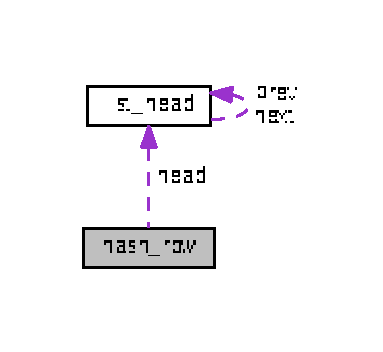
\includegraphics[width=184pt]{structhash__row__coll__graph}
\end{center}
\end{figure}
\subsection*{Public 속성}
\begin{DoxyCompactItemize}
\item 
void $\ast$ \hyperlink{structhash__row_a270cca5040fb8c27a8b5595cc921d960}{p}
\item 
struct \hyperlink{structlist__head}{list\+\_\+head} \hyperlink{structhash__row_aeef0a2f42e9fa516efe336bba7a990d4}{head}
\end{DoxyCompactItemize}


\subsection{멤버 데이타 문서화}
\hypertarget{structhash__row_aeef0a2f42e9fa516efe336bba7a990d4}{\index{hash\+\_\+row@{hash\+\_\+row}!head@{head}}
\index{head@{head}!hash\+\_\+row@{hash\+\_\+row}}
\subsubsection[{head}]{\setlength{\rightskip}{0pt plus 5cm}struct {\bf list\+\_\+head} hash\+\_\+row\+::head}}\label{structhash__row_aeef0a2f42e9fa516efe336bba7a990d4}
\hypertarget{structhash__row_a270cca5040fb8c27a8b5595cc921d960}{\index{hash\+\_\+row@{hash\+\_\+row}!p@{p}}
\index{p@{p}!hash\+\_\+row@{hash\+\_\+row}}
\subsubsection[{p}]{\setlength{\rightskip}{0pt plus 5cm}void$\ast$ hash\+\_\+row\+::p}}\label{structhash__row_a270cca5040fb8c27a8b5595cc921d960}


이 구조체에 대한 문서화 페이지는 다음의 파일로부터 생성되었습니다.\+:\begin{DoxyCompactItemize}
\item 
dkh/\hyperlink{hash_8h}{hash.\+h}\end{DoxyCompactItemize}

\hypertarget{structhash__table}{\section{hash\+\_\+table Struct Reference}
\label{structhash__table}\index{hash\+\_\+table@{hash\+\_\+table}}
}


{\ttfamily \#include $<$hash.\+h$>$}



Collaboration diagram for hash\+\_\+table\+:
\subsection*{Public Attributes}
\begin{DoxyCompactItemize}
\item 
int \hyperlink{structhash__table_a5c37715c358be0aea139f968bd44d3ae}{len}
\item 
struct \hyperlink{structhash__row}{hash\+\_\+row} $\ast$ \hyperlink{structhash__table_a634ff501f78f223799d4923fbcbbf30d}{row}
\end{DoxyCompactItemize}


\subsection{Member Data Documentation}
\hypertarget{structhash__table_a5c37715c358be0aea139f968bd44d3ae}{\index{hash\+\_\+table@{hash\+\_\+table}!len@{len}}
\index{len@{len}!hash\+\_\+table@{hash\+\_\+table}}
\subsubsection[{len}]{\setlength{\rightskip}{0pt plus 5cm}int hash\+\_\+table\+::len}}\label{structhash__table_a5c37715c358be0aea139f968bd44d3ae}
\hypertarget{structhash__table_a634ff501f78f223799d4923fbcbbf30d}{\index{hash\+\_\+table@{hash\+\_\+table}!row@{row}}
\index{row@{row}!hash\+\_\+table@{hash\+\_\+table}}
\subsubsection[{row}]{\setlength{\rightskip}{0pt plus 5cm}struct {\bf hash\+\_\+row}$\ast$ hash\+\_\+table\+::row}}\label{structhash__table_a634ff501f78f223799d4923fbcbbf30d}


The documentation for this struct was generated from the following file\+:\begin{DoxyCompactItemize}
\item 
dkh/\hyperlink{hash_8h}{hash.\+h}\end{DoxyCompactItemize}

\hypertarget{structlist__head}{\section{list\+\_\+head 구조체 참조}
\label{structlist__head}\index{list\+\_\+head@{list\+\_\+head}}
}


{\ttfamily \#include $<$dk\+\_\+list.\+h$>$}



list\+\_\+head에 대한 협력 다이어그램\+:
\nopagebreak
\begin{figure}[H]
\begin{center}
\leavevmode
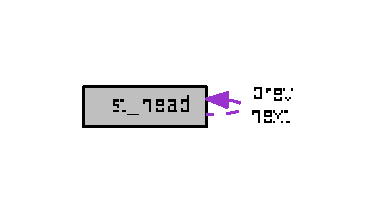
\includegraphics[width=182pt]{structlist__head__coll__graph}
\end{center}
\end{figure}
\subsection*{Public 속성}
\begin{DoxyCompactItemize}
\item 
struct \hyperlink{structlist__head}{list\+\_\+head} $\ast$ \hyperlink{structlist__head_ac3b0ff0dfb978a0cfbdad6b9d19cdcfe}{next}
\item 
struct \hyperlink{structlist__head}{list\+\_\+head} $\ast$ \hyperlink{structlist__head_ae4298f7975979e5f6bb406c40c1fa443}{prev}
\end{DoxyCompactItemize}


\subsection{멤버 데이타 문서화}
\hypertarget{structlist__head_ac3b0ff0dfb978a0cfbdad6b9d19cdcfe}{\index{list\+\_\+head@{list\+\_\+head}!next@{next}}
\index{next@{next}!list\+\_\+head@{list\+\_\+head}}
\subsubsection[{next}]{\setlength{\rightskip}{0pt plus 5cm}struct {\bf list\+\_\+head}$\ast$ list\+\_\+head\+::next}}\label{structlist__head_ac3b0ff0dfb978a0cfbdad6b9d19cdcfe}
\hypertarget{structlist__head_ae4298f7975979e5f6bb406c40c1fa443}{\index{list\+\_\+head@{list\+\_\+head}!prev@{prev}}
\index{prev@{prev}!list\+\_\+head@{list\+\_\+head}}
\subsubsection[{prev}]{\setlength{\rightskip}{0pt plus 5cm}struct {\bf list\+\_\+head}$\ast$ list\+\_\+head\+::prev}}\label{structlist__head_ae4298f7975979e5f6bb406c40c1fa443}


이 구조체에 대한 문서화 페이지는 다음의 파일로부터 생성되었습니다.\+:\begin{DoxyCompactItemize}
\item 
dkh/\hyperlink{dk__list_8h}{dk\+\_\+list.\+h}\end{DoxyCompactItemize}

\hypertarget{structworkload}{\section{workload Struct Reference}
\label{structworkload}\index{workload@{workload}}
}


{\ttfamily \#include $<$lru.\+h$>$}

\subsection*{Public Attributes}
\begin{DoxyCompactItemize}
\item 
char $\ast$ \hyperlink{structworkload_a4401c89ba5cdd383f04301470e163cfd}{time}
\item 
char $\ast$ \hyperlink{structworkload_a3d757b51dfb82980f5a979a97bf0dfa1}{host}
\item 
int \hyperlink{structworkload_ac5fbfd8a1e652dc2b6e742ce685eb1fa}{disk\+\_\+num}
\item 
int \hyperlink{structworkload_aa2845ad1d10cf7ef276771aa7c038c40}{type}
\item 
double \hyperlink{structworkload_a05766e7402dae7d93f0f6602e4498a36}{offset}
\item 
double \hyperlink{structworkload_a5a1b5a6bbc572a36211bb56219e41d2e}{size}
\item 
long \hyperlink{structworkload_a8de001cbb458db8f4502435a2a6c2030}{respone}
\end{DoxyCompactItemize}


\subsection{Member Data Documentation}
\hypertarget{structworkload_ac5fbfd8a1e652dc2b6e742ce685eb1fa}{\index{workload@{workload}!disk\+\_\+num@{disk\+\_\+num}}
\index{disk\+\_\+num@{disk\+\_\+num}!workload@{workload}}
\subsubsection[{disk\+\_\+num}]{\setlength{\rightskip}{0pt plus 5cm}int workload\+::disk\+\_\+num}}\label{structworkload_ac5fbfd8a1e652dc2b6e742ce685eb1fa}
\hypertarget{structworkload_a3d757b51dfb82980f5a979a97bf0dfa1}{\index{workload@{workload}!host@{host}}
\index{host@{host}!workload@{workload}}
\subsubsection[{host}]{\setlength{\rightskip}{0pt plus 5cm}char$\ast$ workload\+::host}}\label{structworkload_a3d757b51dfb82980f5a979a97bf0dfa1}
\hypertarget{structworkload_a05766e7402dae7d93f0f6602e4498a36}{\index{workload@{workload}!offset@{offset}}
\index{offset@{offset}!workload@{workload}}
\subsubsection[{offset}]{\setlength{\rightskip}{0pt plus 5cm}double workload\+::offset}}\label{structworkload_a05766e7402dae7d93f0f6602e4498a36}
\hypertarget{structworkload_a8de001cbb458db8f4502435a2a6c2030}{\index{workload@{workload}!respone@{respone}}
\index{respone@{respone}!workload@{workload}}
\subsubsection[{respone}]{\setlength{\rightskip}{0pt plus 5cm}long workload\+::respone}}\label{structworkload_a8de001cbb458db8f4502435a2a6c2030}
\hypertarget{structworkload_a5a1b5a6bbc572a36211bb56219e41d2e}{\index{workload@{workload}!size@{size}}
\index{size@{size}!workload@{workload}}
\subsubsection[{size}]{\setlength{\rightskip}{0pt plus 5cm}double workload\+::size}}\label{structworkload_a5a1b5a6bbc572a36211bb56219e41d2e}
\hypertarget{structworkload_a4401c89ba5cdd383f04301470e163cfd}{\index{workload@{workload}!time@{time}}
\index{time@{time}!workload@{workload}}
\subsubsection[{time}]{\setlength{\rightskip}{0pt plus 5cm}char$\ast$ workload\+::time}}\label{structworkload_a4401c89ba5cdd383f04301470e163cfd}
\hypertarget{structworkload_aa2845ad1d10cf7ef276771aa7c038c40}{\index{workload@{workload}!type@{type}}
\index{type@{type}!workload@{workload}}
\subsubsection[{type}]{\setlength{\rightskip}{0pt plus 5cm}int workload\+::type}}\label{structworkload_aa2845ad1d10cf7ef276771aa7c038c40}


The documentation for this struct was generated from the following file\+:\begin{DoxyCompactItemize}
\item 
dkh/\hyperlink{lru_8h}{lru.\+h}\end{DoxyCompactItemize}

\chapter{파일 문서화}
\hypertarget{code__analyze_8h}{\section{dkh/code\+\_\+analyze.h 파일 참조}
\label{code__analyze_8h}\index{dkh/code\+\_\+analyze.\+h@{dkh/code\+\_\+analyze.\+h}}
}
{\ttfamily \#include $<$pthread.\+h$>$}\\*
{\ttfamily \#include $<$stdlib.\+h$>$}\\*
{\ttfamily \#include $<$stdio.\+h$>$}\\*
{\ttfamily \#include $<$string.\+h$>$}\\*
{\ttfamily \#include $<$fcntl.\+h$>$}\\*
{\ttfamily \#include $<$sys/syscall.\+h$>$}\\*
{\ttfamily \#include $<$sys/types.\+h$>$}\\*
{\ttfamily \#include \char`\"{}file\+\_\+read.\+h\char`\"{}}\\*
{\ttfamily \#include \char`\"{}print\+\_\+msg.\+h\char`\"{}}\\*
{\ttfamily \#include \char`\"{}dk\+\_\+str.\+h\char`\"{}}\\*
{\ttfamily \#include \char`\"{}dk\+\_\+list.\+h\char`\"{}}\\*
code\+\_\+analyze.\+h에 대한 include 의존 그래프
\nopagebreak
\begin{figure}[H]
\begin{center}
\leavevmode
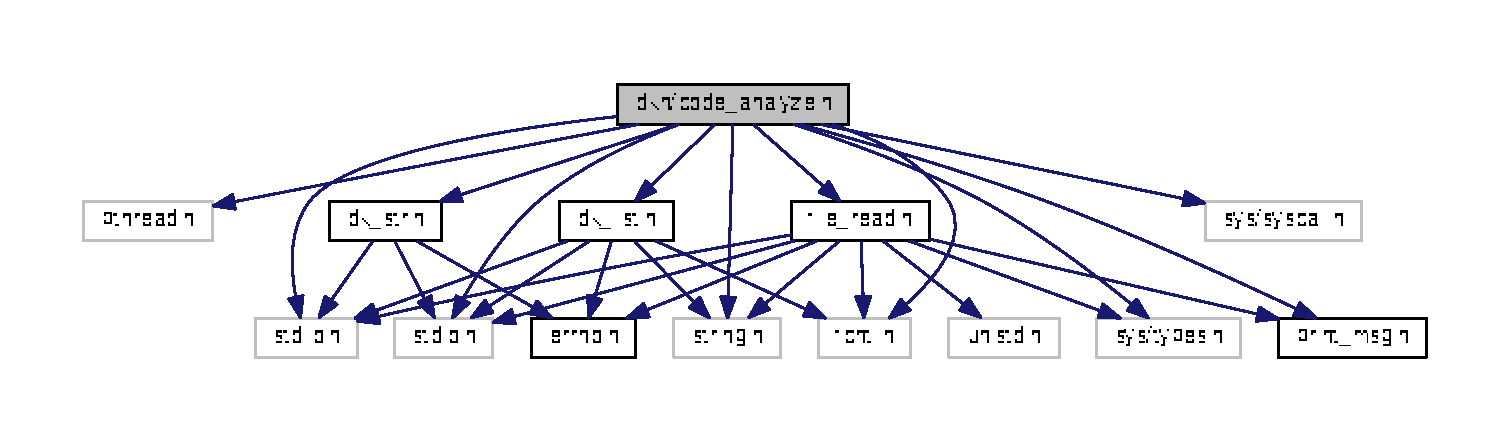
\includegraphics[width=350pt]{code__analyze_8h__incl}
\end{center}
\end{figure}
\subsection*{클래스}
\begin{DoxyCompactItemize}
\item 
struct \hyperlink{structcode__info}{code\+\_\+info}
\item 
struct \hyperlink{structanalysis__arg}{analysis\+\_\+arg}
\end{DoxyCompactItemize}
\subsection*{매크로}
\begin{DoxyCompactItemize}
\item 
\#define \hyperlink{code__analyze_8h_a505e6854b27524988af2985839f53918}{C\+P\+U\+\_\+\+C\+O\+U\+N\+T}~4
\item 
\#define \hyperlink{code__analyze_8h_a98b32c745c3b9c60f87a8e0941a2d934}{K\+E\+Y\+W\+O\+R\+D\+\_\+\+N\+E\+X\+T\+\_\+\+P\+A\+D\+D\+I\+N\+G}~0\+X00000001
\item 
\#define \hyperlink{code__analyze_8h_aaa0a3659a4aca6f6af8fa3a9f91420d4}{K\+E\+Y\+W\+O\+R\+D\+\_\+\+N\+E\+X\+T\+\_\+\+P\+A\+R\+E\+N\+T\+H\+E\+S\+E\+S}~0\+X00000002       /$\ast$ parentheses = '(' or ')' $\ast$/
\item 
\#define \hyperlink{code__analyze_8h_af5c9311183519392f9c326d16c23cc13}{K\+E\+Y\+W\+O\+R\+D\+\_\+\+N\+E\+X\+T\+\_\+\+L\+\_\+\+P\+A\+R\+E\+N\+T\+H\+E\+S\+E\+S}~0\+X00000004     /$\ast$ parentheses = '(' $\ast$/
\item 
\#define \hyperlink{code__analyze_8h_a8c219bbdeb00651c73fe1ce53f67d10c}{K\+E\+Y\+W\+O\+R\+D\+\_\+\+N\+E\+X\+T\+\_\+\+R\+\_\+\+P\+A\+R\+E\+N\+T\+H\+E\+S\+E\+S}~0\+X00000008     /$\ast$ parentheses = ')' $\ast$/
\end{DoxyCompactItemize}
\subsection*{함수}
\begin{DoxyCompactItemize}
\item 
char $\ast$ \hyperlink{code__analyze_8h_a8bd8f2b51bb6544019267bd9e3ced08d}{list\+\_\+str} (struct dk\+\_\+list $\ast$list, char $\ast$str)
\item 
char $\ast$ \hyperlink{code__analyze_8h_ad95127e99785c3217d95e00f8783b444}{cheek\+\_\+code\+\_\+line} (char $\ast$str, struct dk\+\_\+list $\ast$list, int option)
\item 
int \hyperlink{code__analyze_8h_ab121b00ea24f1ab4d78ccae7a343893f}{init\+\_\+code\+\_\+info} (struct \hyperlink{structcode__info}{code\+\_\+info} $\ast$c\+\_\+info, char $\ast$file)
\item 
int $\ast$ \hyperlink{code__analyze_8h_a40c5275f63bcc1394af4771780714285}{read\+\_\+file} (char $\ast$path)
\item 
int \hyperlink{code__analyze_8h_a88d8ed4c2b9673c9fc9f285f09cb3cad}{get\+\_\+file\+\_\+line} (char $\ast$path)
\end{DoxyCompactItemize}


\subsection{매크로 문서화}
\hypertarget{code__analyze_8h_a505e6854b27524988af2985839f53918}{\index{code\+\_\+analyze.\+h@{code\+\_\+analyze.\+h}!C\+P\+U\+\_\+\+C\+O\+U\+N\+T@{C\+P\+U\+\_\+\+C\+O\+U\+N\+T}}
\index{C\+P\+U\+\_\+\+C\+O\+U\+N\+T@{C\+P\+U\+\_\+\+C\+O\+U\+N\+T}!code\+\_\+analyze.\+h@{code\+\_\+analyze.\+h}}
\subsubsection[{C\+P\+U\+\_\+\+C\+O\+U\+N\+T}]{\setlength{\rightskip}{0pt plus 5cm}\#define C\+P\+U\+\_\+\+C\+O\+U\+N\+T~4}}\label{code__analyze_8h_a505e6854b27524988af2985839f53918}
\hypertarget{code__analyze_8h_af5c9311183519392f9c326d16c23cc13}{\index{code\+\_\+analyze.\+h@{code\+\_\+analyze.\+h}!K\+E\+Y\+W\+O\+R\+D\+\_\+\+N\+E\+X\+T\+\_\+\+L\+\_\+\+P\+A\+R\+E\+N\+T\+H\+E\+S\+E\+S@{K\+E\+Y\+W\+O\+R\+D\+\_\+\+N\+E\+X\+T\+\_\+\+L\+\_\+\+P\+A\+R\+E\+N\+T\+H\+E\+S\+E\+S}}
\index{K\+E\+Y\+W\+O\+R\+D\+\_\+\+N\+E\+X\+T\+\_\+\+L\+\_\+\+P\+A\+R\+E\+N\+T\+H\+E\+S\+E\+S@{K\+E\+Y\+W\+O\+R\+D\+\_\+\+N\+E\+X\+T\+\_\+\+L\+\_\+\+P\+A\+R\+E\+N\+T\+H\+E\+S\+E\+S}!code\+\_\+analyze.\+h@{code\+\_\+analyze.\+h}}
\subsubsection[{K\+E\+Y\+W\+O\+R\+D\+\_\+\+N\+E\+X\+T\+\_\+\+L\+\_\+\+P\+A\+R\+E\+N\+T\+H\+E\+S\+E\+S}]{\setlength{\rightskip}{0pt plus 5cm}\#define K\+E\+Y\+W\+O\+R\+D\+\_\+\+N\+E\+X\+T\+\_\+\+L\+\_\+\+P\+A\+R\+E\+N\+T\+H\+E\+S\+E\+S~0\+X00000004     /$\ast$ parentheses = '(' $\ast$/}}\label{code__analyze_8h_af5c9311183519392f9c326d16c23cc13}
\hypertarget{code__analyze_8h_a98b32c745c3b9c60f87a8e0941a2d934}{\index{code\+\_\+analyze.\+h@{code\+\_\+analyze.\+h}!K\+E\+Y\+W\+O\+R\+D\+\_\+\+N\+E\+X\+T\+\_\+\+P\+A\+D\+D\+I\+N\+G@{K\+E\+Y\+W\+O\+R\+D\+\_\+\+N\+E\+X\+T\+\_\+\+P\+A\+D\+D\+I\+N\+G}}
\index{K\+E\+Y\+W\+O\+R\+D\+\_\+\+N\+E\+X\+T\+\_\+\+P\+A\+D\+D\+I\+N\+G@{K\+E\+Y\+W\+O\+R\+D\+\_\+\+N\+E\+X\+T\+\_\+\+P\+A\+D\+D\+I\+N\+G}!code\+\_\+analyze.\+h@{code\+\_\+analyze.\+h}}
\subsubsection[{K\+E\+Y\+W\+O\+R\+D\+\_\+\+N\+E\+X\+T\+\_\+\+P\+A\+D\+D\+I\+N\+G}]{\setlength{\rightskip}{0pt plus 5cm}\#define K\+E\+Y\+W\+O\+R\+D\+\_\+\+N\+E\+X\+T\+\_\+\+P\+A\+D\+D\+I\+N\+G~0\+X00000001}}\label{code__analyze_8h_a98b32c745c3b9c60f87a8e0941a2d934}
\hypertarget{code__analyze_8h_aaa0a3659a4aca6f6af8fa3a9f91420d4}{\index{code\+\_\+analyze.\+h@{code\+\_\+analyze.\+h}!K\+E\+Y\+W\+O\+R\+D\+\_\+\+N\+E\+X\+T\+\_\+\+P\+A\+R\+E\+N\+T\+H\+E\+S\+E\+S@{K\+E\+Y\+W\+O\+R\+D\+\_\+\+N\+E\+X\+T\+\_\+\+P\+A\+R\+E\+N\+T\+H\+E\+S\+E\+S}}
\index{K\+E\+Y\+W\+O\+R\+D\+\_\+\+N\+E\+X\+T\+\_\+\+P\+A\+R\+E\+N\+T\+H\+E\+S\+E\+S@{K\+E\+Y\+W\+O\+R\+D\+\_\+\+N\+E\+X\+T\+\_\+\+P\+A\+R\+E\+N\+T\+H\+E\+S\+E\+S}!code\+\_\+analyze.\+h@{code\+\_\+analyze.\+h}}
\subsubsection[{K\+E\+Y\+W\+O\+R\+D\+\_\+\+N\+E\+X\+T\+\_\+\+P\+A\+R\+E\+N\+T\+H\+E\+S\+E\+S}]{\setlength{\rightskip}{0pt plus 5cm}\#define K\+E\+Y\+W\+O\+R\+D\+\_\+\+N\+E\+X\+T\+\_\+\+P\+A\+R\+E\+N\+T\+H\+E\+S\+E\+S~0\+X00000002       /$\ast$ parentheses = '(' or ')' $\ast$/}}\label{code__analyze_8h_aaa0a3659a4aca6f6af8fa3a9f91420d4}
\hypertarget{code__analyze_8h_a8c219bbdeb00651c73fe1ce53f67d10c}{\index{code\+\_\+analyze.\+h@{code\+\_\+analyze.\+h}!K\+E\+Y\+W\+O\+R\+D\+\_\+\+N\+E\+X\+T\+\_\+\+R\+\_\+\+P\+A\+R\+E\+N\+T\+H\+E\+S\+E\+S@{K\+E\+Y\+W\+O\+R\+D\+\_\+\+N\+E\+X\+T\+\_\+\+R\+\_\+\+P\+A\+R\+E\+N\+T\+H\+E\+S\+E\+S}}
\index{K\+E\+Y\+W\+O\+R\+D\+\_\+\+N\+E\+X\+T\+\_\+\+R\+\_\+\+P\+A\+R\+E\+N\+T\+H\+E\+S\+E\+S@{K\+E\+Y\+W\+O\+R\+D\+\_\+\+N\+E\+X\+T\+\_\+\+R\+\_\+\+P\+A\+R\+E\+N\+T\+H\+E\+S\+E\+S}!code\+\_\+analyze.\+h@{code\+\_\+analyze.\+h}}
\subsubsection[{K\+E\+Y\+W\+O\+R\+D\+\_\+\+N\+E\+X\+T\+\_\+\+R\+\_\+\+P\+A\+R\+E\+N\+T\+H\+E\+S\+E\+S}]{\setlength{\rightskip}{0pt plus 5cm}\#define K\+E\+Y\+W\+O\+R\+D\+\_\+\+N\+E\+X\+T\+\_\+\+R\+\_\+\+P\+A\+R\+E\+N\+T\+H\+E\+S\+E\+S~0\+X00000008     /$\ast$ parentheses = ')' $\ast$/}}\label{code__analyze_8h_a8c219bbdeb00651c73fe1ce53f67d10c}


\subsection{함수 문서화}
\hypertarget{code__analyze_8h_ad95127e99785c3217d95e00f8783b444}{\index{code\+\_\+analyze.\+h@{code\+\_\+analyze.\+h}!cheek\+\_\+code\+\_\+line@{cheek\+\_\+code\+\_\+line}}
\index{cheek\+\_\+code\+\_\+line@{cheek\+\_\+code\+\_\+line}!code\+\_\+analyze.\+h@{code\+\_\+analyze.\+h}}
\subsubsection[{cheek\+\_\+code\+\_\+line}]{\setlength{\rightskip}{0pt plus 5cm}char$\ast$ cheek\+\_\+code\+\_\+line (
\begin{DoxyParamCaption}
\item[{char $\ast$}]{str, }
\item[{struct dk\+\_\+list $\ast$}]{list, }
\item[{int}]{option}
\end{DoxyParamCaption}
)}}\label{code__analyze_8h_ad95127e99785c3217d95e00f8783b444}
\hypertarget{code__analyze_8h_a88d8ed4c2b9673c9fc9f285f09cb3cad}{\index{code\+\_\+analyze.\+h@{code\+\_\+analyze.\+h}!get\+\_\+file\+\_\+line@{get\+\_\+file\+\_\+line}}
\index{get\+\_\+file\+\_\+line@{get\+\_\+file\+\_\+line}!code\+\_\+analyze.\+h@{code\+\_\+analyze.\+h}}
\subsubsection[{get\+\_\+file\+\_\+line}]{\setlength{\rightskip}{0pt plus 5cm}int get\+\_\+file\+\_\+line (
\begin{DoxyParamCaption}
\item[{char $\ast$}]{path}
\end{DoxyParamCaption}
)}}\label{code__analyze_8h_a88d8ed4c2b9673c9fc9f285f09cb3cad}


이 함수 내부에서 호출하는 함수들에 대한 그래프입니다.\+:
\nopagebreak
\begin{figure}[H]
\begin{center}
\leavevmode
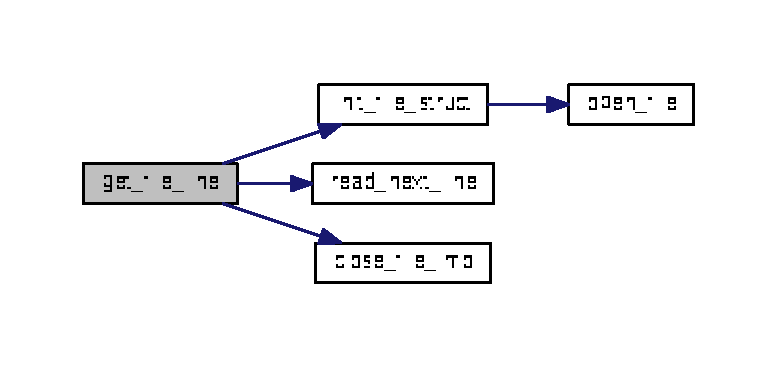
\includegraphics[width=350pt]{code__analyze_8h_a88d8ed4c2b9673c9fc9f285f09cb3cad_cgraph}
\end{center}
\end{figure}


\hypertarget{code__analyze_8h_ab121b00ea24f1ab4d78ccae7a343893f}{\index{code\+\_\+analyze.\+h@{code\+\_\+analyze.\+h}!init\+\_\+code\+\_\+info@{init\+\_\+code\+\_\+info}}
\index{init\+\_\+code\+\_\+info@{init\+\_\+code\+\_\+info}!code\+\_\+analyze.\+h@{code\+\_\+analyze.\+h}}
\subsubsection[{init\+\_\+code\+\_\+info}]{\setlength{\rightskip}{0pt plus 5cm}int init\+\_\+code\+\_\+info (
\begin{DoxyParamCaption}
\item[{struct {\bf code\+\_\+info} $\ast$}]{c\+\_\+info, }
\item[{char $\ast$}]{file}
\end{DoxyParamCaption}
)}}\label{code__analyze_8h_ab121b00ea24f1ab4d78ccae7a343893f}
\hypertarget{code__analyze_8h_a8bd8f2b51bb6544019267bd9e3ced08d}{\index{code\+\_\+analyze.\+h@{code\+\_\+analyze.\+h}!list\+\_\+str@{list\+\_\+str}}
\index{list\+\_\+str@{list\+\_\+str}!code\+\_\+analyze.\+h@{code\+\_\+analyze.\+h}}
\subsubsection[{list\+\_\+str}]{\setlength{\rightskip}{0pt plus 5cm}char$\ast$ list\+\_\+str (
\begin{DoxyParamCaption}
\item[{struct dk\+\_\+list $\ast$}]{list, }
\item[{char $\ast$}]{str}
\end{DoxyParamCaption}
)}}\label{code__analyze_8h_a8bd8f2b51bb6544019267bd9e3ced08d}
\hypertarget{code__analyze_8h_a40c5275f63bcc1394af4771780714285}{\index{code\+\_\+analyze.\+h@{code\+\_\+analyze.\+h}!read\+\_\+file@{read\+\_\+file}}
\index{read\+\_\+file@{read\+\_\+file}!code\+\_\+analyze.\+h@{code\+\_\+analyze.\+h}}
\subsubsection[{read\+\_\+file}]{\setlength{\rightskip}{0pt plus 5cm}int$\ast$ read\+\_\+file (
\begin{DoxyParamCaption}
\item[{char $\ast$}]{path}
\end{DoxyParamCaption}
)}}\label{code__analyze_8h_a40c5275f63bcc1394af4771780714285}


이 함수 내부에서 호출하는 함수들에 대한 그래프입니다.\+:
\nopagebreak
\begin{figure}[H]
\begin{center}
\leavevmode
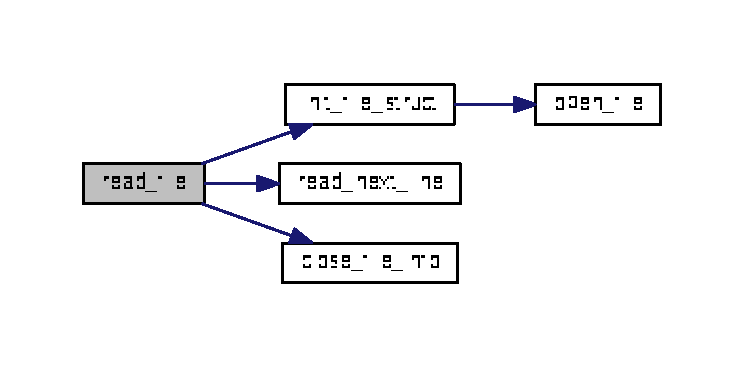
\includegraphics[width=350pt]{code__analyze_8h_a40c5275f63bcc1394af4771780714285_cgraph}
\end{center}
\end{figure}



\hypertarget{compiler_8h}{\section{dkh/compiler.h 파일 참조}
\label{compiler_8h}\index{dkh/compiler.\+h@{dkh/compiler.\+h}}
}
\subsection*{매크로}
\begin{DoxyCompactItemize}
\item 
\#define \hyperlink{compiler_8h_ace6f17999da4ea3b93c4227beafcab95}{\+\_\+\+\_\+user}
\item 
\#define \hyperlink{compiler_8h_a808945c5ae849a5110b6e3127c99023b}{\+\_\+\+\_\+kernel}
\item 
\#define \hyperlink{compiler_8h_a5755174a781f92e269afd3325ac52f13}{\+\_\+\+\_\+safe}
\item 
\#define \hyperlink{compiler_8h_ab95a84e6535084347da05cdf197e045c}{\+\_\+\+\_\+force}
\item 
\#define \hyperlink{compiler_8h_a51428c62a5987efede2308c1161b0a97}{\+\_\+\+\_\+nocast}
\item 
\#define \hyperlink{compiler_8h_af6b4077d1d8ce49175e6fcb91788634a}{\+\_\+\+\_\+iomem}
\item 
\#define \hyperlink{compiler_8h_ab9026ec4a1d5f1b945bcfda44887350f}{\+\_\+\+\_\+chk\+\_\+user\+\_\+ptr}(x)~(void)0
\item 
\#define \hyperlink{compiler_8h_a4d1c02e76cb441be40c0b3b2105f08c8}{\+\_\+\+\_\+chk\+\_\+io\+\_\+ptr}(x)~(void)0
\item 
\#define \hyperlink{compiler_8h_abd682821c58566962421c62b3ce99588}{\+\_\+\+\_\+builtin\+\_\+warning}(x, y...)~(1)
\item 
\#define \hyperlink{compiler_8h_a6bc6af579890d9cfaa45b8487b130166}{\+\_\+\+\_\+acquires}(x)
\item 
\#define \hyperlink{compiler_8h_a8a48e2e572ccda0f5dcf0af7c4bf9d6c}{\+\_\+\+\_\+releases}(x)
\item 
\#define \hyperlink{compiler_8h_a09350f685c337603efd490a82b896a3b}{\+\_\+\+\_\+acquire}(x)~(void)0
\item 
\#define \hyperlink{compiler_8h_a33f52bd22e55cd51cb5092be21d1e6f5}{\+\_\+\+\_\+release}(x)~(void)0
\item 
\#define \hyperlink{compiler_8h_a8608d9f2a737b9640fea72932d0c0841}{\+\_\+\+\_\+cond\+\_\+lock}(x, c)~(c)
\item 
\#define \hyperlink{compiler_8h_abea77661c5bf0bc3e4cf992f84a42c5b}{\+\_\+\+\_\+attribute\+\_\+const\+\_\+\+\_\+}~/$\ast$ unimplemented $\ast$/
\item 
\#define \hyperlink{compiler_8h_af74f8ba1e24b5ef7ab220682dd106e37}{\+\_\+\+\_\+cold}
\end{DoxyCompactItemize}


\subsection{매크로 문서화}
\hypertarget{compiler_8h_a09350f685c337603efd490a82b896a3b}{\index{compiler.\+h@{compiler.\+h}!\+\_\+\+\_\+acquire@{\+\_\+\+\_\+acquire}}
\index{\+\_\+\+\_\+acquire@{\+\_\+\+\_\+acquire}!compiler.\+h@{compiler.\+h}}
\subsubsection[{\+\_\+\+\_\+acquire}]{\setlength{\rightskip}{0pt plus 5cm}\#define \+\_\+\+\_\+acquire(
\begin{DoxyParamCaption}
\item[{}]{x}
\end{DoxyParamCaption}
)~(void)0}}\label{compiler_8h_a09350f685c337603efd490a82b896a3b}
\hypertarget{compiler_8h_a6bc6af579890d9cfaa45b8487b130166}{\index{compiler.\+h@{compiler.\+h}!\+\_\+\+\_\+acquires@{\+\_\+\+\_\+acquires}}
\index{\+\_\+\+\_\+acquires@{\+\_\+\+\_\+acquires}!compiler.\+h@{compiler.\+h}}
\subsubsection[{\+\_\+\+\_\+acquires}]{\setlength{\rightskip}{0pt plus 5cm}\#define \+\_\+\+\_\+acquires(
\begin{DoxyParamCaption}
\item[{}]{x}
\end{DoxyParamCaption}
)}}\label{compiler_8h_a6bc6af579890d9cfaa45b8487b130166}
\hypertarget{compiler_8h_abea77661c5bf0bc3e4cf992f84a42c5b}{\index{compiler.\+h@{compiler.\+h}!\+\_\+\+\_\+attribute\+\_\+const\+\_\+\+\_\+@{\+\_\+\+\_\+attribute\+\_\+const\+\_\+\+\_\+}}
\index{\+\_\+\+\_\+attribute\+\_\+const\+\_\+\+\_\+@{\+\_\+\+\_\+attribute\+\_\+const\+\_\+\+\_\+}!compiler.\+h@{compiler.\+h}}
\subsubsection[{\+\_\+\+\_\+attribute\+\_\+const\+\_\+\+\_\+}]{\setlength{\rightskip}{0pt plus 5cm}\#define \+\_\+\+\_\+attribute\+\_\+const\+\_\+\+\_\+~/$\ast$ unimplemented $\ast$/}}\label{compiler_8h_abea77661c5bf0bc3e4cf992f84a42c5b}
\hypertarget{compiler_8h_abd682821c58566962421c62b3ce99588}{\index{compiler.\+h@{compiler.\+h}!\+\_\+\+\_\+builtin\+\_\+warning@{\+\_\+\+\_\+builtin\+\_\+warning}}
\index{\+\_\+\+\_\+builtin\+\_\+warning@{\+\_\+\+\_\+builtin\+\_\+warning}!compiler.\+h@{compiler.\+h}}
\subsubsection[{\+\_\+\+\_\+builtin\+\_\+warning}]{\setlength{\rightskip}{0pt plus 5cm}\#define \+\_\+\+\_\+builtin\+\_\+warning(
\begin{DoxyParamCaption}
\item[{}]{x, }
\item[{}]{y...}
\end{DoxyParamCaption}
)~(1)}}\label{compiler_8h_abd682821c58566962421c62b3ce99588}
\hypertarget{compiler_8h_a4d1c02e76cb441be40c0b3b2105f08c8}{\index{compiler.\+h@{compiler.\+h}!\+\_\+\+\_\+chk\+\_\+io\+\_\+ptr@{\+\_\+\+\_\+chk\+\_\+io\+\_\+ptr}}
\index{\+\_\+\+\_\+chk\+\_\+io\+\_\+ptr@{\+\_\+\+\_\+chk\+\_\+io\+\_\+ptr}!compiler.\+h@{compiler.\+h}}
\subsubsection[{\+\_\+\+\_\+chk\+\_\+io\+\_\+ptr}]{\setlength{\rightskip}{0pt plus 5cm}\#define \+\_\+\+\_\+chk\+\_\+io\+\_\+ptr(
\begin{DoxyParamCaption}
\item[{}]{x}
\end{DoxyParamCaption}
)~(void)0}}\label{compiler_8h_a4d1c02e76cb441be40c0b3b2105f08c8}
\hypertarget{compiler_8h_ab9026ec4a1d5f1b945bcfda44887350f}{\index{compiler.\+h@{compiler.\+h}!\+\_\+\+\_\+chk\+\_\+user\+\_\+ptr@{\+\_\+\+\_\+chk\+\_\+user\+\_\+ptr}}
\index{\+\_\+\+\_\+chk\+\_\+user\+\_\+ptr@{\+\_\+\+\_\+chk\+\_\+user\+\_\+ptr}!compiler.\+h@{compiler.\+h}}
\subsubsection[{\+\_\+\+\_\+chk\+\_\+user\+\_\+ptr}]{\setlength{\rightskip}{0pt plus 5cm}\#define \+\_\+\+\_\+chk\+\_\+user\+\_\+ptr(
\begin{DoxyParamCaption}
\item[{}]{x}
\end{DoxyParamCaption}
)~(void)0}}\label{compiler_8h_ab9026ec4a1d5f1b945bcfda44887350f}
\hypertarget{compiler_8h_af74f8ba1e24b5ef7ab220682dd106e37}{\index{compiler.\+h@{compiler.\+h}!\+\_\+\+\_\+cold@{\+\_\+\+\_\+cold}}
\index{\+\_\+\+\_\+cold@{\+\_\+\+\_\+cold}!compiler.\+h@{compiler.\+h}}
\subsubsection[{\+\_\+\+\_\+cold}]{\setlength{\rightskip}{0pt plus 5cm}\#define \+\_\+\+\_\+cold}}\label{compiler_8h_af74f8ba1e24b5ef7ab220682dd106e37}
\hypertarget{compiler_8h_a8608d9f2a737b9640fea72932d0c0841}{\index{compiler.\+h@{compiler.\+h}!\+\_\+\+\_\+cond\+\_\+lock@{\+\_\+\+\_\+cond\+\_\+lock}}
\index{\+\_\+\+\_\+cond\+\_\+lock@{\+\_\+\+\_\+cond\+\_\+lock}!compiler.\+h@{compiler.\+h}}
\subsubsection[{\+\_\+\+\_\+cond\+\_\+lock}]{\setlength{\rightskip}{0pt plus 5cm}\#define \+\_\+\+\_\+cond\+\_\+lock(
\begin{DoxyParamCaption}
\item[{}]{x, }
\item[{}]{c}
\end{DoxyParamCaption}
)~(c)}}\label{compiler_8h_a8608d9f2a737b9640fea72932d0c0841}
\hypertarget{compiler_8h_ab95a84e6535084347da05cdf197e045c}{\index{compiler.\+h@{compiler.\+h}!\+\_\+\+\_\+force@{\+\_\+\+\_\+force}}
\index{\+\_\+\+\_\+force@{\+\_\+\+\_\+force}!compiler.\+h@{compiler.\+h}}
\subsubsection[{\+\_\+\+\_\+force}]{\setlength{\rightskip}{0pt plus 5cm}\#define \+\_\+\+\_\+force}}\label{compiler_8h_ab95a84e6535084347da05cdf197e045c}
\hypertarget{compiler_8h_af6b4077d1d8ce49175e6fcb91788634a}{\index{compiler.\+h@{compiler.\+h}!\+\_\+\+\_\+iomem@{\+\_\+\+\_\+iomem}}
\index{\+\_\+\+\_\+iomem@{\+\_\+\+\_\+iomem}!compiler.\+h@{compiler.\+h}}
\subsubsection[{\+\_\+\+\_\+iomem}]{\setlength{\rightskip}{0pt plus 5cm}\#define \+\_\+\+\_\+iomem}}\label{compiler_8h_af6b4077d1d8ce49175e6fcb91788634a}
\hypertarget{compiler_8h_a808945c5ae849a5110b6e3127c99023b}{\index{compiler.\+h@{compiler.\+h}!\+\_\+\+\_\+kernel@{\+\_\+\+\_\+kernel}}
\index{\+\_\+\+\_\+kernel@{\+\_\+\+\_\+kernel}!compiler.\+h@{compiler.\+h}}
\subsubsection[{\+\_\+\+\_\+kernel}]{\setlength{\rightskip}{0pt plus 5cm}\#define \+\_\+\+\_\+kernel}}\label{compiler_8h_a808945c5ae849a5110b6e3127c99023b}
\hypertarget{compiler_8h_a51428c62a5987efede2308c1161b0a97}{\index{compiler.\+h@{compiler.\+h}!\+\_\+\+\_\+nocast@{\+\_\+\+\_\+nocast}}
\index{\+\_\+\+\_\+nocast@{\+\_\+\+\_\+nocast}!compiler.\+h@{compiler.\+h}}
\subsubsection[{\+\_\+\+\_\+nocast}]{\setlength{\rightskip}{0pt plus 5cm}\#define \+\_\+\+\_\+nocast}}\label{compiler_8h_a51428c62a5987efede2308c1161b0a97}
\hypertarget{compiler_8h_a33f52bd22e55cd51cb5092be21d1e6f5}{\index{compiler.\+h@{compiler.\+h}!\+\_\+\+\_\+release@{\+\_\+\+\_\+release}}
\index{\+\_\+\+\_\+release@{\+\_\+\+\_\+release}!compiler.\+h@{compiler.\+h}}
\subsubsection[{\+\_\+\+\_\+release}]{\setlength{\rightskip}{0pt plus 5cm}\#define \+\_\+\+\_\+release(
\begin{DoxyParamCaption}
\item[{}]{x}
\end{DoxyParamCaption}
)~(void)0}}\label{compiler_8h_a33f52bd22e55cd51cb5092be21d1e6f5}
\hypertarget{compiler_8h_a8a48e2e572ccda0f5dcf0af7c4bf9d6c}{\index{compiler.\+h@{compiler.\+h}!\+\_\+\+\_\+releases@{\+\_\+\+\_\+releases}}
\index{\+\_\+\+\_\+releases@{\+\_\+\+\_\+releases}!compiler.\+h@{compiler.\+h}}
\subsubsection[{\+\_\+\+\_\+releases}]{\setlength{\rightskip}{0pt plus 5cm}\#define \+\_\+\+\_\+releases(
\begin{DoxyParamCaption}
\item[{}]{x}
\end{DoxyParamCaption}
)}}\label{compiler_8h_a8a48e2e572ccda0f5dcf0af7c4bf9d6c}
\hypertarget{compiler_8h_a5755174a781f92e269afd3325ac52f13}{\index{compiler.\+h@{compiler.\+h}!\+\_\+\+\_\+safe@{\+\_\+\+\_\+safe}}
\index{\+\_\+\+\_\+safe@{\+\_\+\+\_\+safe}!compiler.\+h@{compiler.\+h}}
\subsubsection[{\+\_\+\+\_\+safe}]{\setlength{\rightskip}{0pt plus 5cm}\#define \+\_\+\+\_\+safe}}\label{compiler_8h_a5755174a781f92e269afd3325ac52f13}
\hypertarget{compiler_8h_ace6f17999da4ea3b93c4227beafcab95}{\index{compiler.\+h@{compiler.\+h}!\+\_\+\+\_\+user@{\+\_\+\+\_\+user}}
\index{\+\_\+\+\_\+user@{\+\_\+\+\_\+user}!compiler.\+h@{compiler.\+h}}
\subsubsection[{\+\_\+\+\_\+user}]{\setlength{\rightskip}{0pt plus 5cm}\#define \+\_\+\+\_\+user}}\label{compiler_8h_ace6f17999da4ea3b93c4227beafcab95}

\hypertarget{dk__kernel_8h}{\section{dkh/dk\+\_\+kernel.h File Reference}
\label{dk__kernel_8h}\index{dkh/dk\+\_\+kernel.\+h@{dkh/dk\+\_\+kernel.\+h}}
}
\subsection*{Macros}
\begin{DoxyCompactItemize}
\item 
\#define \hyperlink{dk__kernel_8h_ad89ebe5fe5ad08c683f0871118ea8e2f}{offsetof}(s, m)~(size\+\_\+t)\&(((s $\ast$)0)-\/$>$m)
\item 
\#define \hyperlink{dk__kernel_8h_af8c317a42292b61c93aae91e59118a46}{container\+\_\+of}(ptr, type, member)
\end{DoxyCompactItemize}


\subsection{Macro Definition Documentation}
\hypertarget{dk__kernel_8h_af8c317a42292b61c93aae91e59118a46}{\index{dk\+\_\+kernel.\+h@{dk\+\_\+kernel.\+h}!container\+\_\+of@{container\+\_\+of}}
\index{container\+\_\+of@{container\+\_\+of}!dk\+\_\+kernel.\+h@{dk\+\_\+kernel.\+h}}
\subsubsection[{container\+\_\+of}]{\setlength{\rightskip}{0pt plus 5cm}\#define container\+\_\+of(
\begin{DoxyParamCaption}
\item[{}]{ptr, }
\item[{}]{type, }
\item[{}]{member}
\end{DoxyParamCaption}
)}}\label{dk__kernel_8h_af8c317a42292b61c93aae91e59118a46}
{\bfseries Value\+:}
\begin{DoxyCode}
(\{                      \(\backslash\)
            const typeof( ((\hyperlink{structworkload_aa2845ad1d10cf7ef276771aa7c038c40}{type} *)0)->member ) *\_\_mptr = (ptr);    \(\backslash\)
            (\hyperlink{structworkload_aa2845ad1d10cf7ef276771aa7c038c40}{type} *)( (\textcolor{keywordtype}{char} *)\_\_mptr - \hyperlink{dk__kernel_8h_ad89ebe5fe5ad08c683f0871118ea8e2f}{offsetof}(\hyperlink{structworkload_aa2845ad1d10cf7ef276771aa7c038c40}{type},member) );\})
\end{DoxyCode}
\hypertarget{dk__kernel_8h_ad89ebe5fe5ad08c683f0871118ea8e2f}{\index{dk\+\_\+kernel.\+h@{dk\+\_\+kernel.\+h}!offsetof@{offsetof}}
\index{offsetof@{offsetof}!dk\+\_\+kernel.\+h@{dk\+\_\+kernel.\+h}}
\subsubsection[{offsetof}]{\setlength{\rightskip}{0pt plus 5cm}\#define offsetof(
\begin{DoxyParamCaption}
\item[{}]{s, }
\item[{}]{m}
\end{DoxyParamCaption}
)~(size\+\_\+t)\&(((s $\ast$)0)-\/$>$m)}}\label{dk__kernel_8h_ad89ebe5fe5ad08c683f0871118ea8e2f}

\hypertarget{dk__list_8h}{\section{dkh/dk\+\_\+list.h File Reference}
\label{dk__list_8h}\index{dkh/dk\+\_\+list.\+h@{dkh/dk\+\_\+list.\+h}}
}
{\ttfamily \#include $<$stdlib.\+h$>$}\\*
{\ttfamily \#include $<$stdio.\+h$>$}\\*
{\ttfamily \#include $<$string.\+h$>$}\\*
{\ttfamily \#include $<$fcntl.\+h$>$}\\*
{\ttfamily \#include \char`\"{}errno.\+h\char`\"{}}\\*
Include dependency graph for dk\+\_\+list.\+h\+:
This graph shows which files directly or indirectly include this file\+:
\subsection*{Classes}
\begin{DoxyCompactItemize}
\item 
struct \hyperlink{structlist__head}{list\+\_\+head}
\end{DoxyCompactItemize}
\subsection*{Macros}
\begin{DoxyCompactItemize}
\item 
\#define \hyperlink{dk__list_8h_afd049f7ad59dbe455f460807475c2841}{offsetof}(type, member)~((size\+\_\+t) \&((type $\ast$)0)-\/$>$member)
\item 
\#define \hyperlink{dk__list_8h_af8c317a42292b61c93aae91e59118a46}{container\+\_\+of}(ptr, type, member)
\item 
\#define \hyperlink{dk__list_8h_ab8b24e6660ab3760c923e4b4db3fa502}{list\+\_\+for\+\_\+each}(pos, head)
\end{DoxyCompactItemize}
\subsection*{Functions}
\begin{DoxyCompactItemize}
\item 
struct \hyperlink{structlist__head}{list\+\_\+head} $\ast$ \hyperlink{dk__list_8h_a3ea33987d84e227c8398958e10a10bbd}{init\+\_\+lnode} ()
\item 
void \hyperlink{dk__list_8h_a742e4907797f8815f3f519518dbfa4cd}{print\+\_\+node} (struct \hyperlink{structlist__head}{list\+\_\+head} $\ast$n)
\end{DoxyCompactItemize}


\subsection{Macro Definition Documentation}
\hypertarget{dk__list_8h_af8c317a42292b61c93aae91e59118a46}{\index{dk\+\_\+list.\+h@{dk\+\_\+list.\+h}!container\+\_\+of@{container\+\_\+of}}
\index{container\+\_\+of@{container\+\_\+of}!dk\+\_\+list.\+h@{dk\+\_\+list.\+h}}
\subsubsection[{container\+\_\+of}]{\setlength{\rightskip}{0pt plus 5cm}\#define container\+\_\+of(
\begin{DoxyParamCaption}
\item[{}]{ptr, }
\item[{}]{type, }
\item[{}]{member}
\end{DoxyParamCaption}
)}}\label{dk__list_8h_af8c317a42292b61c93aae91e59118a46}
{\bfseries Value\+:}
\begin{DoxyCode}
(\{\(\backslash\)
    const typeof( ((\hyperlink{structworkload_aa2845ad1d10cf7ef276771aa7c038c40}{type} *)0)->member ) *\_\_mptr = (ptr);\(\backslash\)
    (\hyperlink{structworkload_aa2845ad1d10cf7ef276771aa7c038c40}{type} *)( (\textcolor{keywordtype}{char} *)\_\_mptr - \hyperlink{dk__list_8h_afd049f7ad59dbe455f460807475c2841}{offsetof}(\hyperlink{structworkload_aa2845ad1d10cf7ef276771aa7c038c40}{type},member) );\})
\end{DoxyCode}
\hypertarget{dk__list_8h_ab8b24e6660ab3760c923e4b4db3fa502}{\index{dk\+\_\+list.\+h@{dk\+\_\+list.\+h}!list\+\_\+for\+\_\+each@{list\+\_\+for\+\_\+each}}
\index{list\+\_\+for\+\_\+each@{list\+\_\+for\+\_\+each}!dk\+\_\+list.\+h@{dk\+\_\+list.\+h}}
\subsubsection[{list\+\_\+for\+\_\+each}]{\setlength{\rightskip}{0pt plus 5cm}\#define list\+\_\+for\+\_\+each(
\begin{DoxyParamCaption}
\item[{}]{pos, }
\item[{}]{head}
\end{DoxyParamCaption}
)}}\label{dk__list_8h_ab8b24e6660ab3760c923e4b4db3fa502}
{\bfseries Value\+:}
\begin{DoxyCode}
\textcolor{keywordflow}{for} (pos = (head)->next; prefetch(pos->next), pos != (head); \(\backslash\)
      pos = pos->next)
\end{DoxyCode}
\hypertarget{dk__list_8h_afd049f7ad59dbe455f460807475c2841}{\index{dk\+\_\+list.\+h@{dk\+\_\+list.\+h}!offsetof@{offsetof}}
\index{offsetof@{offsetof}!dk\+\_\+list.\+h@{dk\+\_\+list.\+h}}
\subsubsection[{offsetof}]{\setlength{\rightskip}{0pt plus 5cm}\#define offsetof(
\begin{DoxyParamCaption}
\item[{}]{type, }
\item[{}]{member}
\end{DoxyParamCaption}
)~((size\+\_\+t) \&((type $\ast$)0)-\/$>$member)}}\label{dk__list_8h_afd049f7ad59dbe455f460807475c2841}


\subsection{Function Documentation}
\hypertarget{dk__list_8h_a3ea33987d84e227c8398958e10a10bbd}{\index{dk\+\_\+list.\+h@{dk\+\_\+list.\+h}!init\+\_\+lnode@{init\+\_\+lnode}}
\index{init\+\_\+lnode@{init\+\_\+lnode}!dk\+\_\+list.\+h@{dk\+\_\+list.\+h}}
\subsubsection[{init\+\_\+lnode}]{\setlength{\rightskip}{0pt plus 5cm}struct {\bf list\+\_\+head}$\ast$ init\+\_\+lnode (
\begin{DoxyParamCaption}
{}
\end{DoxyParamCaption}
)}}\label{dk__list_8h_a3ea33987d84e227c8398958e10a10bbd}


Here is the caller graph for this function\+:


\hypertarget{dk__list_8h_a742e4907797f8815f3f519518dbfa4cd}{\index{dk\+\_\+list.\+h@{dk\+\_\+list.\+h}!print\+\_\+node@{print\+\_\+node}}
\index{print\+\_\+node@{print\+\_\+node}!dk\+\_\+list.\+h@{dk\+\_\+list.\+h}}
\subsubsection[{print\+\_\+node}]{\setlength{\rightskip}{0pt plus 5cm}void print\+\_\+node (
\begin{DoxyParamCaption}
\item[{struct {\bf list\+\_\+head} $\ast$}]{n}
\end{DoxyParamCaption}
)\hspace{0.3cm}{\ttfamily [inline]}}}\label{dk__list_8h_a742e4907797f8815f3f519518dbfa4cd}

\hypertarget{dk__str_8h}{\section{dkh/dk\+\_\+str.h 파일 참조}
\label{dk__str_8h}\index{dkh/dk\+\_\+str.\+h@{dkh/dk\+\_\+str.\+h}}
}
{\ttfamily \#include $<$stdlib.\+h$>$}\\*
{\ttfamily \#include $<$stdio.\+h$>$}\\*
{\ttfamily \#include \char`\"{}errno.\+h\char`\"{}}\\*
dk\+\_\+str.\+h에 대한 include 의존 그래프
\nopagebreak
\begin{figure}[H]
\begin{center}
\leavevmode
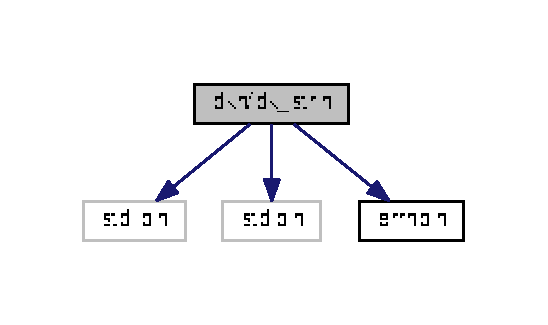
\includegraphics[width=263pt]{dk__str_8h__incl}
\end{center}
\end{figure}
이 그래프는 이 파일을 직/간접적으로 include 하는 파일들을 보여줍니다.\+:
\nopagebreak
\begin{figure}[H]
\begin{center}
\leavevmode
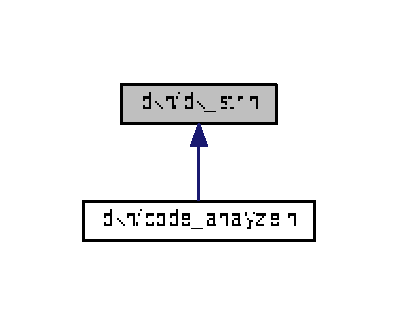
\includegraphics[width=191pt]{dk__str_8h__dep__incl}
\end{center}
\end{figure}
\subsection*{함수}
\begin{DoxyCompactItemize}
\item 
int \hyperlink{dk__str_8h_a3e5d14083c3345b0142058e26571046e}{str\+\_\+contain} (char $\ast$str, char c)
\end{DoxyCompactItemize}


\subsection{함수 문서화}
\hypertarget{dk__str_8h_a3e5d14083c3345b0142058e26571046e}{\index{dk\+\_\+str.\+h@{dk\+\_\+str.\+h}!str\+\_\+contain@{str\+\_\+contain}}
\index{str\+\_\+contain@{str\+\_\+contain}!dk\+\_\+str.\+h@{dk\+\_\+str.\+h}}
\subsubsection[{str\+\_\+contain}]{\setlength{\rightskip}{0pt plus 5cm}int str\+\_\+contain (
\begin{DoxyParamCaption}
\item[{char $\ast$}]{str, }
\item[{char}]{c}
\end{DoxyParamCaption}
)}}\label{dk__str_8h_a3e5d14083c3345b0142058e26571046e}

\hypertarget{dk__tree_8h}{\section{dkh/dk\+\_\+tree.h 파일 참조}
\label{dk__tree_8h}\index{dkh/dk\+\_\+tree.\+h@{dkh/dk\+\_\+tree.\+h}}
}
{\ttfamily \#include $<$stdlib.\+h$>$}\\*
{\ttfamily \#include $<$stdio.\+h$>$}\\*
{\ttfamily \#include $<$string.\+h$>$}\\*
{\ttfamily \#include $<$fcntl.\+h$>$}\\*
{\ttfamily \#include \char`\"{}errno.\+h\char`\"{}}\\*
dk\+\_\+tree.\+h에 대한 include 의존 그래프
\nopagebreak
\begin{figure}[H]
\begin{center}
\leavevmode
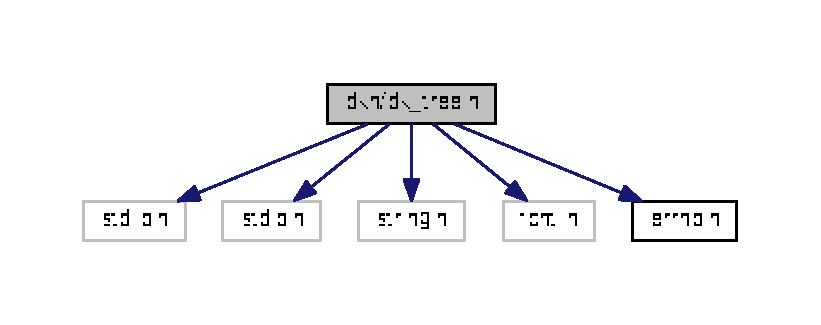
\includegraphics[width=350pt]{dk__tree_8h__incl}
\end{center}
\end{figure}
\subsection*{클래스}
\begin{DoxyCompactItemize}
\item 
struct \hyperlink{structdk__tree}{dk\+\_\+tree}
\item 
struct \hyperlink{structdk__tnode}{dk\+\_\+tnode}
\end{DoxyCompactItemize}
\subsection*{함수}
\begin{DoxyCompactItemize}
\item 
struct \hyperlink{structdk__tnode}{dk\+\_\+tnode} $\ast$ \hyperlink{dk__tree_8h_a7b04e296ac39a39b21f53bd8d2d0d396}{init\+\_\+tnode} (void $\ast$val)
\item 
struct \hyperlink{structdk__tree}{dk\+\_\+tree} $\ast$ \hyperlink{dk__tree_8h_a17447454787f220fa813c211f7a9eedd}{init\+\_\+tree} (void)
\item 
void \hyperlink{dk__tree_8h_adde758b473e6652d4754ca62de435021}{print\+\_\+tnode} (struct \hyperlink{structdk__tnode}{dk\+\_\+tnode} $\ast$n)
\item 
struct \hyperlink{structdk__tnode}{dk\+\_\+tnode} $\ast$ \hyperlink{dk__tree_8h_acaec7c2d143007a2e9bdd3b9f7def467}{add\+\_\+tnode} (struct \hyperlink{structdk__tree}{dk\+\_\+tree} $\ast$tree, char $\ast$c)
\end{DoxyCompactItemize}


\subsection{함수 문서화}
\hypertarget{dk__tree_8h_acaec7c2d143007a2e9bdd3b9f7def467}{\index{dk\+\_\+tree.\+h@{dk\+\_\+tree.\+h}!add\+\_\+tnode@{add\+\_\+tnode}}
\index{add\+\_\+tnode@{add\+\_\+tnode}!dk\+\_\+tree.\+h@{dk\+\_\+tree.\+h}}
\subsubsection[{add\+\_\+tnode}]{\setlength{\rightskip}{0pt plus 5cm}struct {\bf dk\+\_\+tnode}$\ast$ add\+\_\+tnode (
\begin{DoxyParamCaption}
\item[{struct {\bf dk\+\_\+tree} $\ast$}]{tree, }
\item[{char $\ast$}]{c}
\end{DoxyParamCaption}
)}}\label{dk__tree_8h_acaec7c2d143007a2e9bdd3b9f7def467}


이 함수 내부에서 호출하는 함수들에 대한 그래프입니다.\+:
\nopagebreak
\begin{figure}[H]
\begin{center}
\leavevmode
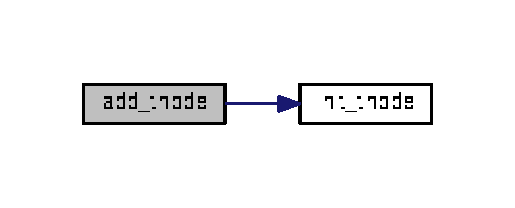
\includegraphics[width=247pt]{dk__tree_8h_acaec7c2d143007a2e9bdd3b9f7def467_cgraph}
\end{center}
\end{figure}


\hypertarget{dk__tree_8h_a7b04e296ac39a39b21f53bd8d2d0d396}{\index{dk\+\_\+tree.\+h@{dk\+\_\+tree.\+h}!init\+\_\+tnode@{init\+\_\+tnode}}
\index{init\+\_\+tnode@{init\+\_\+tnode}!dk\+\_\+tree.\+h@{dk\+\_\+tree.\+h}}
\subsubsection[{init\+\_\+tnode}]{\setlength{\rightskip}{0pt plus 5cm}struct {\bf dk\+\_\+tnode}$\ast$ init\+\_\+tnode (
\begin{DoxyParamCaption}
\item[{void $\ast$}]{val}
\end{DoxyParamCaption}
)}}\label{dk__tree_8h_a7b04e296ac39a39b21f53bd8d2d0d396}


이 함수를 호출하는 함수들에 대한 그래프입니다.\+:
\nopagebreak
\begin{figure}[H]
\begin{center}
\leavevmode
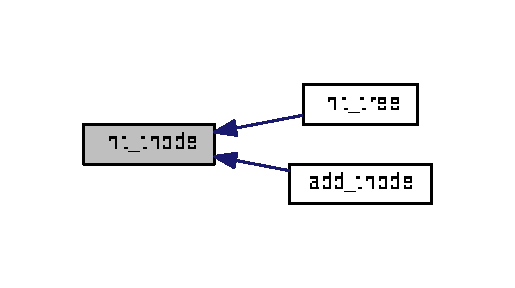
\includegraphics[width=247pt]{dk__tree_8h_a7b04e296ac39a39b21f53bd8d2d0d396_icgraph}
\end{center}
\end{figure}


\hypertarget{dk__tree_8h_a17447454787f220fa813c211f7a9eedd}{\index{dk\+\_\+tree.\+h@{dk\+\_\+tree.\+h}!init\+\_\+tree@{init\+\_\+tree}}
\index{init\+\_\+tree@{init\+\_\+tree}!dk\+\_\+tree.\+h@{dk\+\_\+tree.\+h}}
\subsubsection[{init\+\_\+tree}]{\setlength{\rightskip}{0pt plus 5cm}struct {\bf dk\+\_\+tree}$\ast$ init\+\_\+tree (
\begin{DoxyParamCaption}
\item[{void}]{}
\end{DoxyParamCaption}
)}}\label{dk__tree_8h_a17447454787f220fa813c211f7a9eedd}


이 함수 내부에서 호출하는 함수들에 대한 그래프입니다.\+:
\nopagebreak
\begin{figure}[H]
\begin{center}
\leavevmode
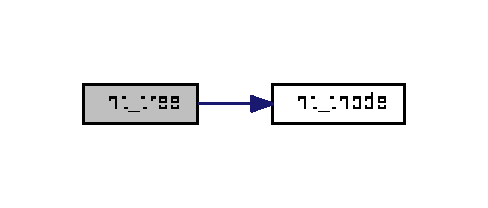
\includegraphics[width=234pt]{dk__tree_8h_a17447454787f220fa813c211f7a9eedd_cgraph}
\end{center}
\end{figure}


\hypertarget{dk__tree_8h_adde758b473e6652d4754ca62de435021}{\index{dk\+\_\+tree.\+h@{dk\+\_\+tree.\+h}!print\+\_\+tnode@{print\+\_\+tnode}}
\index{print\+\_\+tnode@{print\+\_\+tnode}!dk\+\_\+tree.\+h@{dk\+\_\+tree.\+h}}
\subsubsection[{print\+\_\+tnode}]{\setlength{\rightskip}{0pt plus 5cm}void print\+\_\+tnode (
\begin{DoxyParamCaption}
\item[{struct {\bf dk\+\_\+tnode} $\ast$}]{n}
\end{DoxyParamCaption}
)\hspace{0.3cm}{\ttfamily [inline]}}}\label{dk__tree_8h_adde758b473e6652d4754ca62de435021}

\hypertarget{errno_8h}{\section{dkh/errno.h File Reference}
\label{errno_8h}\index{dkh/errno.\+h@{dkh/errno.\+h}}
}
This graph shows which files directly or indirectly include this file\+:
\subsection*{Macros}
\begin{DoxyCompactItemize}
\item 
\#define \hyperlink{errno_8h_afd07dee740688463691d16fa242d4dd4}{E\+A\+R\+G\+\_\+\+N\+U\+L\+L}~-\/0x0000001
\end{DoxyCompactItemize}


\subsection{Macro Definition Documentation}
\hypertarget{errno_8h_afd07dee740688463691d16fa242d4dd4}{\index{errno.\+h@{errno.\+h}!E\+A\+R\+G\+\_\+\+N\+U\+L\+L@{E\+A\+R\+G\+\_\+\+N\+U\+L\+L}}
\index{E\+A\+R\+G\+\_\+\+N\+U\+L\+L@{E\+A\+R\+G\+\_\+\+N\+U\+L\+L}!errno.\+h@{errno.\+h}}
\subsubsection[{E\+A\+R\+G\+\_\+\+N\+U\+L\+L}]{\setlength{\rightskip}{0pt plus 5cm}\#define E\+A\+R\+G\+\_\+\+N\+U\+L\+L~-\/0x0000001}}\label{errno_8h_afd07dee740688463691d16fa242d4dd4}

\hypertarget{file__read_8h}{\section{dkh/file\+\_\+read.h File Reference}
\label{file__read_8h}\index{dkh/file\+\_\+read.\+h@{dkh/file\+\_\+read.\+h}}
}
{\ttfamily \#include $<$stdlib.\+h$>$}\\*
{\ttfamily \#include $<$stdio.\+h$>$}\\*
{\ttfamily \#include $<$string.\+h$>$}\\*
{\ttfamily \#include $<$fcntl.\+h$>$}\\*
{\ttfamily \#include $<$sys/types.\+h$>$}\\*
{\ttfamily \#include $<$unistd.\+h$>$}\\*
{\ttfamily \#include \char`\"{}errno.\+h\char`\"{}}\\*
{\ttfamily \#include \char`\"{}print\+\_\+msg.\+h\char`\"{}}\\*
Include dependency graph for file\+\_\+read.\+h\+:
This graph shows which files directly or indirectly include this file\+:
\subsection*{Classes}
\begin{DoxyCompactItemize}
\item 
struct \hyperlink{structfile__info}{file\+\_\+info}
\end{DoxyCompactItemize}
\subsection*{Macros}
\begin{DoxyCompactItemize}
\item 
\#define \hyperlink{file__read_8h_a212979f5fc9dcf0a420e90b9b21d780a}{M\+A\+X\+\_\+\+B\+U\+F\+F\+\_\+\+S\+I\+Z\+E}~1024 $\ast$ 1024 $\ast$ 4
\end{DoxyCompactItemize}
\subsection*{Functions}
\begin{DoxyCompactItemize}
\item 
int \hyperlink{file__read_8h_ad36ccbba17c95e2853bf8bd7a6346eaa}{init\+\_\+file\+\_\+struct} (struct \hyperlink{structfile__info}{file\+\_\+info} $\ast$info, char $\ast$path)
\item 
int \hyperlink{file__read_8h_ae84bfdae0ec7b73cf580228efa76178e}{open\+\_\+file} (char $\ast$path)
\item 
int \hyperlink{file__read_8h_ae31df81b043dc729e24b00b2797fd601}{close\+\_\+file\+\_\+info} (struct \hyperlink{structfile__info}{file\+\_\+info} $\ast$s)
\item 
char $\ast$ \hyperlink{file__read_8h_a6ca2c59b960803be2495125fd8ad9ee9}{read\+\_\+token\+\_\+line} (struct \hyperlink{structfile__info}{file\+\_\+info} $\ast$info, int column, char token)
\item 
int \hyperlink{file__read_8h_ac7079eec938e493fb76cd68e9b86b176}{next\+\_\+buff\+\_\+read\+\_\+seek} (struct \hyperlink{structfile__info}{file\+\_\+info} $\ast$info, int rb)
\item 
int \hyperlink{file__read_8h_a8f0aa9ed68fd12c76459bd21b090cf44}{next\+\_\+buff\+\_\+read} (struct \hyperlink{structfile__info}{file\+\_\+info} $\ast$info)
\item 
char $\ast$ \hyperlink{file__read_8h_a744a461bab4a6c47c93cc697a3464761}{read\+\_\+next\+\_\+line} (struct \hyperlink{structfile__info}{file\+\_\+info} $\ast$info)
\end{DoxyCompactItemize}


\subsection{Macro Definition Documentation}
\hypertarget{file__read_8h_a212979f5fc9dcf0a420e90b9b21d780a}{\index{file\+\_\+read.\+h@{file\+\_\+read.\+h}!M\+A\+X\+\_\+\+B\+U\+F\+F\+\_\+\+S\+I\+Z\+E@{M\+A\+X\+\_\+\+B\+U\+F\+F\+\_\+\+S\+I\+Z\+E}}
\index{M\+A\+X\+\_\+\+B\+U\+F\+F\+\_\+\+S\+I\+Z\+E@{M\+A\+X\+\_\+\+B\+U\+F\+F\+\_\+\+S\+I\+Z\+E}!file\+\_\+read.\+h@{file\+\_\+read.\+h}}
\subsubsection[{M\+A\+X\+\_\+\+B\+U\+F\+F\+\_\+\+S\+I\+Z\+E}]{\setlength{\rightskip}{0pt plus 5cm}\#define M\+A\+X\+\_\+\+B\+U\+F\+F\+\_\+\+S\+I\+Z\+E~1024 $\ast$ 1024 $\ast$ 4}}\label{file__read_8h_a212979f5fc9dcf0a420e90b9b21d780a}


\subsection{Function Documentation}
\hypertarget{file__read_8h_ae31df81b043dc729e24b00b2797fd601}{\index{file\+\_\+read.\+h@{file\+\_\+read.\+h}!close\+\_\+file\+\_\+info@{close\+\_\+file\+\_\+info}}
\index{close\+\_\+file\+\_\+info@{close\+\_\+file\+\_\+info}!file\+\_\+read.\+h@{file\+\_\+read.\+h}}
\subsubsection[{close\+\_\+file\+\_\+info}]{\setlength{\rightskip}{0pt plus 5cm}int close\+\_\+file\+\_\+info (
\begin{DoxyParamCaption}
\item[{struct {\bf file\+\_\+info} $\ast$}]{s}
\end{DoxyParamCaption}
)}}\label{file__read_8h_ae31df81b043dc729e24b00b2797fd601}


Here is the caller graph for this function\+:


\hypertarget{file__read_8h_ad36ccbba17c95e2853bf8bd7a6346eaa}{\index{file\+\_\+read.\+h@{file\+\_\+read.\+h}!init\+\_\+file\+\_\+struct@{init\+\_\+file\+\_\+struct}}
\index{init\+\_\+file\+\_\+struct@{init\+\_\+file\+\_\+struct}!file\+\_\+read.\+h@{file\+\_\+read.\+h}}
\subsubsection[{init\+\_\+file\+\_\+struct}]{\setlength{\rightskip}{0pt plus 5cm}int init\+\_\+file\+\_\+struct (
\begin{DoxyParamCaption}
\item[{struct {\bf file\+\_\+info} $\ast$}]{info, }
\item[{char $\ast$}]{path}
\end{DoxyParamCaption}
)}}\label{file__read_8h_ad36ccbba17c95e2853bf8bd7a6346eaa}


Here is the call graph for this function\+:




Here is the caller graph for this function\+:


\hypertarget{file__read_8h_a8f0aa9ed68fd12c76459bd21b090cf44}{\index{file\+\_\+read.\+h@{file\+\_\+read.\+h}!next\+\_\+buff\+\_\+read@{next\+\_\+buff\+\_\+read}}
\index{next\+\_\+buff\+\_\+read@{next\+\_\+buff\+\_\+read}!file\+\_\+read.\+h@{file\+\_\+read.\+h}}
\subsubsection[{next\+\_\+buff\+\_\+read}]{\setlength{\rightskip}{0pt plus 5cm}int next\+\_\+buff\+\_\+read (
\begin{DoxyParamCaption}
\item[{struct {\bf file\+\_\+info} $\ast$}]{info}
\end{DoxyParamCaption}
)}}\label{file__read_8h_a8f0aa9ed68fd12c76459bd21b090cf44}
\hypertarget{file__read_8h_ac7079eec938e493fb76cd68e9b86b176}{\index{file\+\_\+read.\+h@{file\+\_\+read.\+h}!next\+\_\+buff\+\_\+read\+\_\+seek@{next\+\_\+buff\+\_\+read\+\_\+seek}}
\index{next\+\_\+buff\+\_\+read\+\_\+seek@{next\+\_\+buff\+\_\+read\+\_\+seek}!file\+\_\+read.\+h@{file\+\_\+read.\+h}}
\subsubsection[{next\+\_\+buff\+\_\+read\+\_\+seek}]{\setlength{\rightskip}{0pt plus 5cm}int next\+\_\+buff\+\_\+read\+\_\+seek (
\begin{DoxyParamCaption}
\item[{struct {\bf file\+\_\+info} $\ast$}]{info, }
\item[{int}]{rb}
\end{DoxyParamCaption}
)}}\label{file__read_8h_ac7079eec938e493fb76cd68e9b86b176}
\hypertarget{file__read_8h_ae84bfdae0ec7b73cf580228efa76178e}{\index{file\+\_\+read.\+h@{file\+\_\+read.\+h}!open\+\_\+file@{open\+\_\+file}}
\index{open\+\_\+file@{open\+\_\+file}!file\+\_\+read.\+h@{file\+\_\+read.\+h}}
\subsubsection[{open\+\_\+file}]{\setlength{\rightskip}{0pt plus 5cm}int open\+\_\+file (
\begin{DoxyParamCaption}
\item[{char $\ast$}]{path}
\end{DoxyParamCaption}
)}}\label{file__read_8h_ae84bfdae0ec7b73cf580228efa76178e}


Here is the caller graph for this function\+:


\hypertarget{file__read_8h_a744a461bab4a6c47c93cc697a3464761}{\index{file\+\_\+read.\+h@{file\+\_\+read.\+h}!read\+\_\+next\+\_\+line@{read\+\_\+next\+\_\+line}}
\index{read\+\_\+next\+\_\+line@{read\+\_\+next\+\_\+line}!file\+\_\+read.\+h@{file\+\_\+read.\+h}}
\subsubsection[{read\+\_\+next\+\_\+line}]{\setlength{\rightskip}{0pt plus 5cm}char$\ast$ read\+\_\+next\+\_\+line (
\begin{DoxyParamCaption}
\item[{struct {\bf file\+\_\+info} $\ast$}]{info}
\end{DoxyParamCaption}
)}}\label{file__read_8h_a744a461bab4a6c47c93cc697a3464761}


Here is the caller graph for this function\+:


\hypertarget{file__read_8h_a6ca2c59b960803be2495125fd8ad9ee9}{\index{file\+\_\+read.\+h@{file\+\_\+read.\+h}!read\+\_\+token\+\_\+line@{read\+\_\+token\+\_\+line}}
\index{read\+\_\+token\+\_\+line@{read\+\_\+token\+\_\+line}!file\+\_\+read.\+h@{file\+\_\+read.\+h}}
\subsubsection[{read\+\_\+token\+\_\+line}]{\setlength{\rightskip}{0pt plus 5cm}char$\ast$ read\+\_\+token\+\_\+line (
\begin{DoxyParamCaption}
\item[{struct {\bf file\+\_\+info} $\ast$}]{info, }
\item[{int}]{column, }
\item[{char}]{token}
\end{DoxyParamCaption}
)}}\label{file__read_8h_a6ca2c59b960803be2495125fd8ad9ee9}

\hypertarget{hash_8h}{\section{dkh/hash.h 파일 참조}
\label{hash_8h}\index{dkh/hash.\+h@{dkh/hash.\+h}}
}
{\ttfamily \#include \char`\"{}dk\+\_\+list.\+h\char`\"{}}\\*
hash.\+h에 대한 include 의존 그래프
\nopagebreak
\begin{figure}[H]
\begin{center}
\leavevmode
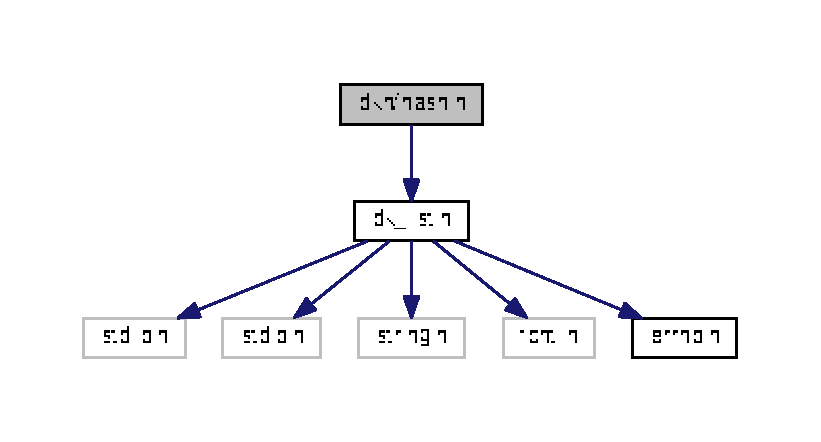
\includegraphics[width=350pt]{hash_8h__incl}
\end{center}
\end{figure}
이 그래프는 이 파일을 직/간접적으로 include 하는 파일들을 보여줍니다.\+:
\nopagebreak
\begin{figure}[H]
\begin{center}
\leavevmode
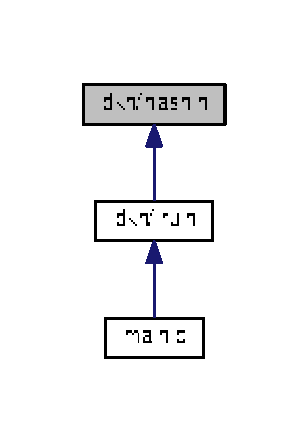
\includegraphics[width=148pt]{hash_8h__dep__incl}
\end{center}
\end{figure}
\subsection*{클래스}
\begin{DoxyCompactItemize}
\item 
struct \hyperlink{structhash__row}{hash\+\_\+row}
\item 
struct \hyperlink{structhash__table}{hash\+\_\+table}
\end{DoxyCompactItemize}
\subsection*{매크로}
\begin{DoxyCompactItemize}
\item 
\#define \hyperlink{hash_8h_afd3853249b57c6560440603a83d1b536}{G\+O\+L\+D\+E\+N\+\_\+\+R\+A\+T\+I\+O\+\_\+\+P\+R\+I\+M\+E\+\_\+32}~0x9e370001\+U\+L
\end{DoxyCompactItemize}
\subsection*{함수}
\begin{DoxyCompactItemize}
\item 
int \hyperlink{hash_8h_ac0ed02b6da15aa5d9f3133e17e456f5a}{add\+\_\+hash\+\_\+table} (struct \hyperlink{structhash__table}{hash\+\_\+table} $\ast$ht, unsigned int val)
\item 
int \hyperlink{hash_8h_ac54ac030e7a4006a06178388a72aa43a}{lookup\+\_\+hash} (struct \hyperlink{structhash__table}{hash\+\_\+table} $\ast$ht)
\item 
struct \hyperlink{structhash__table}{hash\+\_\+table} $\ast$ \hyperlink{hash_8h_acd06af48c2cda8ad19417a6eb1bbe191}{init\+\_\+hash} (int len)
\end{DoxyCompactItemize}


\subsection{매크로 문서화}
\hypertarget{hash_8h_afd3853249b57c6560440603a83d1b536}{\index{hash.\+h@{hash.\+h}!G\+O\+L\+D\+E\+N\+\_\+\+R\+A\+T\+I\+O\+\_\+\+P\+R\+I\+M\+E\+\_\+32@{G\+O\+L\+D\+E\+N\+\_\+\+R\+A\+T\+I\+O\+\_\+\+P\+R\+I\+M\+E\+\_\+32}}
\index{G\+O\+L\+D\+E\+N\+\_\+\+R\+A\+T\+I\+O\+\_\+\+P\+R\+I\+M\+E\+\_\+32@{G\+O\+L\+D\+E\+N\+\_\+\+R\+A\+T\+I\+O\+\_\+\+P\+R\+I\+M\+E\+\_\+32}!hash.\+h@{hash.\+h}}
\subsubsection[{G\+O\+L\+D\+E\+N\+\_\+\+R\+A\+T\+I\+O\+\_\+\+P\+R\+I\+M\+E\+\_\+32}]{\setlength{\rightskip}{0pt plus 5cm}\#define G\+O\+L\+D\+E\+N\+\_\+\+R\+A\+T\+I\+O\+\_\+\+P\+R\+I\+M\+E\+\_\+32~0x9e370001\+U\+L}}\label{hash_8h_afd3853249b57c6560440603a83d1b536}


\subsection{함수 문서화}
\hypertarget{hash_8h_ac0ed02b6da15aa5d9f3133e17e456f5a}{\index{hash.\+h@{hash.\+h}!add\+\_\+hash\+\_\+table@{add\+\_\+hash\+\_\+table}}
\index{add\+\_\+hash\+\_\+table@{add\+\_\+hash\+\_\+table}!hash.\+h@{hash.\+h}}
\subsubsection[{add\+\_\+hash\+\_\+table}]{\setlength{\rightskip}{0pt plus 5cm}int add\+\_\+hash\+\_\+table (
\begin{DoxyParamCaption}
\item[{struct {\bf hash\+\_\+table} $\ast$}]{ht, }
\item[{unsigned int}]{val}
\end{DoxyParamCaption}
)}}\label{hash_8h_ac0ed02b6da15aa5d9f3133e17e456f5a}
\hypertarget{hash_8h_acd06af48c2cda8ad19417a6eb1bbe191}{\index{hash.\+h@{hash.\+h}!init\+\_\+hash@{init\+\_\+hash}}
\index{init\+\_\+hash@{init\+\_\+hash}!hash.\+h@{hash.\+h}}
\subsubsection[{init\+\_\+hash}]{\setlength{\rightskip}{0pt plus 5cm}struct {\bf hash\+\_\+table}$\ast$ init\+\_\+hash (
\begin{DoxyParamCaption}
\item[{int}]{len}
\end{DoxyParamCaption}
)}}\label{hash_8h_acd06af48c2cda8ad19417a6eb1bbe191}
\hypertarget{hash_8h_ac54ac030e7a4006a06178388a72aa43a}{\index{hash.\+h@{hash.\+h}!lookup\+\_\+hash@{lookup\+\_\+hash}}
\index{lookup\+\_\+hash@{lookup\+\_\+hash}!hash.\+h@{hash.\+h}}
\subsubsection[{lookup\+\_\+hash}]{\setlength{\rightskip}{0pt plus 5cm}int lookup\+\_\+hash (
\begin{DoxyParamCaption}
\item[{struct {\bf hash\+\_\+table} $\ast$}]{ht}
\end{DoxyParamCaption}
)}}\label{hash_8h_ac54ac030e7a4006a06178388a72aa43a}

\hypertarget{list_8h}{\section{dkh/list.h 파일 참조}
\label{list_8h}\index{dkh/list.\+h@{dkh/list.\+h}}
}

\hypertarget{lru_8h}{\section{dkh/lru.h File Reference}
\label{lru_8h}\index{dkh/lru.\+h@{dkh/lru.\+h}}
}
{\ttfamily \#include \char`\"{}hash.\+h\char`\"{}}\\*
{\ttfamily \#include $<$math.\+h$>$}\\*
Include dependency graph for lru.\+h\+:
This graph shows which files directly or indirectly include this file\+:
\subsection*{Classes}
\begin{DoxyCompactItemize}
\item 
struct \hyperlink{structworkload}{workload}
\item 
struct \hyperlink{structcache__line}{cache\+\_\+line}
\item 
struct \hyperlink{structcache__mem}{cache\+\_\+mem}
\end{DoxyCompactItemize}
\subsection*{Macros}
\begin{DoxyCompactItemize}
\item 
\#define \hyperlink{lru_8h_ada74e7db007a68e763f20c17f2985356}{R\+E\+A\+D}~1
\item 
\#define \hyperlink{lru_8h_aa10f470e996d0f51210d24f442d25e1e}{W\+R\+I\+T\+E}~2
\item 
\#define \hyperlink{lru_8h_a1841fd1a462d245d8c73dce55e2f45da}{K\+B}~(1024)
\item 
\#define \hyperlink{lru_8h_aa6b38d492364d98453284934ed7caee9}{M\+B}~(\hyperlink{lru_8h_a1841fd1a462d245d8c73dce55e2f45da}{K\+B} $\ast$ \hyperlink{lru_8h_a1841fd1a462d245d8c73dce55e2f45da}{K\+B})
\item 
\#define \hyperlink{lru_8h_a44172ac633c517cb4c9e278cef36b000}{G\+B}~(\hyperlink{lru_8h_aa6b38d492364d98453284934ed7caee9}{M\+B} $\ast$ \hyperlink{lru_8h_a1841fd1a462d245d8c73dce55e2f45da}{K\+B})
\item 
\#define \hyperlink{lru_8h_a9e92828e1e7a7cc03003c00282384f96}{C\+A\+C\+H\+E\+\_\+\+B\+L\+O\+C\+K\+\_\+\+S\+I\+Z\+E}~(4 $\ast$ \hyperlink{lru_8h_a1841fd1a462d245d8c73dce55e2f45da}{K\+B})
\item 
\#define \hyperlink{lru_8h_a8a6befd630ea1c2ab260266f7466540c}{C\+A\+C\+H\+E\+\_\+\+S\+I\+Z\+E}~(64 $\ast$ \hyperlink{lru_8h_aa6b38d492364d98453284934ed7caee9}{M\+B})
\item 
\#define \hyperlink{lru_8h_a5f235d9e65a9cf74d98a037841b04f42}{C\+A\+C\+H\+E\+\_\+\+L\+E\+N}~(\hyperlink{lru_8h_a8a6befd630ea1c2ab260266f7466540c}{C\+A\+C\+H\+E\+\_\+\+S\+I\+Z\+E}/ \hyperlink{lru_8h_a9e92828e1e7a7cc03003c00282384f96}{C\+A\+C\+H\+E\+\_\+\+B\+L\+O\+C\+K\+\_\+\+S\+I\+Z\+E})
\item 
\#define \hyperlink{lru_8h_ae596a4581aaa87caa5cfc716730adaa1}{D\+E\+B\+U\+G\+\_\+\+O\+P\+T\+I\+O\+N}~0
\end{DoxyCompactItemize}
\subsection*{Functions}
\begin{DoxyCompactItemize}
\item 
struct \hyperlink{structcache__mem}{cache\+\_\+mem} $\ast$ \hyperlink{lru_8h_a97ee2a27cdbe15463e52c1b0606cbd1a}{init\+\_\+cache\+\_\+mem} (long m)
\item 
void \hyperlink{lru_8h_a987168b3169b138b36aad5903e5ce4ee}{report\+\_\+cm} (struct \hyperlink{structcache__mem}{cache\+\_\+mem} $\ast$cm)
\item 
int \hyperlink{lru_8h_a8cc95bde93b57fde8f83927b3fd8cca4}{print\+\_\+cm} (struct \hyperlink{structcache__mem}{cache\+\_\+mem} $\ast$cm)
\item 
int \hyperlink{lru_8h_a66199de61dbaaf537f67a7308c0d89d6}{L\+R\+U\+\_\+read} (struct \hyperlink{structcache__mem}{cache\+\_\+mem} $\ast$cm, double line)
\item 
int \hyperlink{lru_8h_a40eb25ee3a00dd9d6371a9f96ba7568b}{L\+R\+U\+\_\+write} (struct \hyperlink{structcache__mem}{cache\+\_\+mem} $\ast$cm, double line)
\item 
int \hyperlink{lru_8h_a3d667614dda729b6e0491823d5e8b3d1}{run\+\_\+cache} (struct \hyperlink{structcache__mem}{cache\+\_\+mem} $\ast$cm, struct \hyperlink{structworkload}{workload} $\ast$wl)
\item 
F\+I\+L\+E $\ast$ \hyperlink{lru_8h_a18d6e93c1f872081867eee56e7d943f7}{open\+\_\+workload} (char $\ast$file)
\item 
int \hyperlink{lru_8h_a30c6287565ac5b2d5161a0642c59888a}{read\+\_\+column} (struct \hyperlink{structworkload}{workload} $\ast$wl, char $\ast$buf)
\item 
int \hyperlink{lru_8h_a23bbdc4f3ff2ccbf5aaf6a2cc5a584b8}{read\+\_\+workload} (struct \hyperlink{structworkload}{workload} $\ast$wl, F\+I\+L\+E $\ast$fp)
\end{DoxyCompactItemize}


\subsection{Detailed Description}
===================================================================================== \begin{DoxyVerb}  Filename:  lru.h

  @date    2004/11/21
  @author  dkdk
\end{DoxyVerb}


Description\+: \begin{DoxyVerb}Version:  1.0
Created:  2014년 10월 26일 03시 43분 37초
\end{DoxyVerb}
 Revision\+: none Compiler\+: gcc

author\+: Jun-\/hyung Park organization\+: Dankook U\+N\+I\+V. 



\subsection{Macro Definition Documentation}
\hypertarget{lru_8h_a9e92828e1e7a7cc03003c00282384f96}{\index{lru.\+h@{lru.\+h}!C\+A\+C\+H\+E\+\_\+\+B\+L\+O\+C\+K\+\_\+\+S\+I\+Z\+E@{C\+A\+C\+H\+E\+\_\+\+B\+L\+O\+C\+K\+\_\+\+S\+I\+Z\+E}}
\index{C\+A\+C\+H\+E\+\_\+\+B\+L\+O\+C\+K\+\_\+\+S\+I\+Z\+E@{C\+A\+C\+H\+E\+\_\+\+B\+L\+O\+C\+K\+\_\+\+S\+I\+Z\+E}!lru.\+h@{lru.\+h}}
\subsubsection[{C\+A\+C\+H\+E\+\_\+\+B\+L\+O\+C\+K\+\_\+\+S\+I\+Z\+E}]{\setlength{\rightskip}{0pt plus 5cm}\#define C\+A\+C\+H\+E\+\_\+\+B\+L\+O\+C\+K\+\_\+\+S\+I\+Z\+E~(4 $\ast$ {\bf K\+B})}}\label{lru_8h_a9e92828e1e7a7cc03003c00282384f96}
\hypertarget{lru_8h_a5f235d9e65a9cf74d98a037841b04f42}{\index{lru.\+h@{lru.\+h}!C\+A\+C\+H\+E\+\_\+\+L\+E\+N@{C\+A\+C\+H\+E\+\_\+\+L\+E\+N}}
\index{C\+A\+C\+H\+E\+\_\+\+L\+E\+N@{C\+A\+C\+H\+E\+\_\+\+L\+E\+N}!lru.\+h@{lru.\+h}}
\subsubsection[{C\+A\+C\+H\+E\+\_\+\+L\+E\+N}]{\setlength{\rightskip}{0pt plus 5cm}\#define C\+A\+C\+H\+E\+\_\+\+L\+E\+N~({\bf C\+A\+C\+H\+E\+\_\+\+S\+I\+Z\+E}/ {\bf C\+A\+C\+H\+E\+\_\+\+B\+L\+O\+C\+K\+\_\+\+S\+I\+Z\+E})}}\label{lru_8h_a5f235d9e65a9cf74d98a037841b04f42}
\hypertarget{lru_8h_a8a6befd630ea1c2ab260266f7466540c}{\index{lru.\+h@{lru.\+h}!C\+A\+C\+H\+E\+\_\+\+S\+I\+Z\+E@{C\+A\+C\+H\+E\+\_\+\+S\+I\+Z\+E}}
\index{C\+A\+C\+H\+E\+\_\+\+S\+I\+Z\+E@{C\+A\+C\+H\+E\+\_\+\+S\+I\+Z\+E}!lru.\+h@{lru.\+h}}
\subsubsection[{C\+A\+C\+H\+E\+\_\+\+S\+I\+Z\+E}]{\setlength{\rightskip}{0pt plus 5cm}\#define C\+A\+C\+H\+E\+\_\+\+S\+I\+Z\+E~(64 $\ast$ {\bf M\+B})}}\label{lru_8h_a8a6befd630ea1c2ab260266f7466540c}
\hypertarget{lru_8h_ae596a4581aaa87caa5cfc716730adaa1}{\index{lru.\+h@{lru.\+h}!D\+E\+B\+U\+G\+\_\+\+O\+P\+T\+I\+O\+N@{D\+E\+B\+U\+G\+\_\+\+O\+P\+T\+I\+O\+N}}
\index{D\+E\+B\+U\+G\+\_\+\+O\+P\+T\+I\+O\+N@{D\+E\+B\+U\+G\+\_\+\+O\+P\+T\+I\+O\+N}!lru.\+h@{lru.\+h}}
\subsubsection[{D\+E\+B\+U\+G\+\_\+\+O\+P\+T\+I\+O\+N}]{\setlength{\rightskip}{0pt plus 5cm}\#define D\+E\+B\+U\+G\+\_\+\+O\+P\+T\+I\+O\+N~0}}\label{lru_8h_ae596a4581aaa87caa5cfc716730adaa1}
\hypertarget{lru_8h_a44172ac633c517cb4c9e278cef36b000}{\index{lru.\+h@{lru.\+h}!G\+B@{G\+B}}
\index{G\+B@{G\+B}!lru.\+h@{lru.\+h}}
\subsubsection[{G\+B}]{\setlength{\rightskip}{0pt plus 5cm}\#define G\+B~({\bf M\+B} $\ast$ {\bf K\+B})}}\label{lru_8h_a44172ac633c517cb4c9e278cef36b000}
\hypertarget{lru_8h_a1841fd1a462d245d8c73dce55e2f45da}{\index{lru.\+h@{lru.\+h}!K\+B@{K\+B}}
\index{K\+B@{K\+B}!lru.\+h@{lru.\+h}}
\subsubsection[{K\+B}]{\setlength{\rightskip}{0pt plus 5cm}\#define K\+B~(1024)}}\label{lru_8h_a1841fd1a462d245d8c73dce55e2f45da}
\hypertarget{lru_8h_aa6b38d492364d98453284934ed7caee9}{\index{lru.\+h@{lru.\+h}!M\+B@{M\+B}}
\index{M\+B@{M\+B}!lru.\+h@{lru.\+h}}
\subsubsection[{M\+B}]{\setlength{\rightskip}{0pt plus 5cm}\#define M\+B~({\bf K\+B} $\ast$ {\bf K\+B})}}\label{lru_8h_aa6b38d492364d98453284934ed7caee9}
\hypertarget{lru_8h_ada74e7db007a68e763f20c17f2985356}{\index{lru.\+h@{lru.\+h}!R\+E\+A\+D@{R\+E\+A\+D}}
\index{R\+E\+A\+D@{R\+E\+A\+D}!lru.\+h@{lru.\+h}}
\subsubsection[{R\+E\+A\+D}]{\setlength{\rightskip}{0pt plus 5cm}\#define R\+E\+A\+D~1}}\label{lru_8h_ada74e7db007a68e763f20c17f2985356}
\hypertarget{lru_8h_aa10f470e996d0f51210d24f442d25e1e}{\index{lru.\+h@{lru.\+h}!W\+R\+I\+T\+E@{W\+R\+I\+T\+E}}
\index{W\+R\+I\+T\+E@{W\+R\+I\+T\+E}!lru.\+h@{lru.\+h}}
\subsubsection[{W\+R\+I\+T\+E}]{\setlength{\rightskip}{0pt plus 5cm}\#define W\+R\+I\+T\+E~2}}\label{lru_8h_aa10f470e996d0f51210d24f442d25e1e}


\subsection{Function Documentation}
\hypertarget{lru_8h_a97ee2a27cdbe15463e52c1b0606cbd1a}{\index{lru.\+h@{lru.\+h}!init\+\_\+cache\+\_\+mem@{init\+\_\+cache\+\_\+mem}}
\index{init\+\_\+cache\+\_\+mem@{init\+\_\+cache\+\_\+mem}!lru.\+h@{lru.\+h}}
\subsubsection[{init\+\_\+cache\+\_\+mem}]{\setlength{\rightskip}{0pt plus 5cm}struct {\bf cache\+\_\+mem}$\ast$ init\+\_\+cache\+\_\+mem (
\begin{DoxyParamCaption}
\item[{long}]{m}
\end{DoxyParamCaption}
)}}\label{lru_8h_a97ee2a27cdbe15463e52c1b0606cbd1a}


Here is the call graph for this function\+:




Here is the caller graph for this function\+:


\hypertarget{lru_8h_a66199de61dbaaf537f67a7308c0d89d6}{\index{lru.\+h@{lru.\+h}!L\+R\+U\+\_\+read@{L\+R\+U\+\_\+read}}
\index{L\+R\+U\+\_\+read@{L\+R\+U\+\_\+read}!lru.\+h@{lru.\+h}}
\subsubsection[{L\+R\+U\+\_\+read}]{\setlength{\rightskip}{0pt plus 5cm}int L\+R\+U\+\_\+read (
\begin{DoxyParamCaption}
\item[{struct {\bf cache\+\_\+mem} $\ast$}]{cm, }
\item[{double}]{line}
\end{DoxyParamCaption}
)}}\label{lru_8h_a66199de61dbaaf537f67a7308c0d89d6}
\hypertarget{lru_8h_a40eb25ee3a00dd9d6371a9f96ba7568b}{\index{lru.\+h@{lru.\+h}!L\+R\+U\+\_\+write@{L\+R\+U\+\_\+write}}
\index{L\+R\+U\+\_\+write@{L\+R\+U\+\_\+write}!lru.\+h@{lru.\+h}}
\subsubsection[{L\+R\+U\+\_\+write}]{\setlength{\rightskip}{0pt plus 5cm}int L\+R\+U\+\_\+write (
\begin{DoxyParamCaption}
\item[{struct {\bf cache\+\_\+mem} $\ast$}]{cm, }
\item[{double}]{line}
\end{DoxyParamCaption}
)}}\label{lru_8h_a40eb25ee3a00dd9d6371a9f96ba7568b}


Here is the call graph for this function\+:




Here is the caller graph for this function\+:


\hypertarget{lru_8h_a18d6e93c1f872081867eee56e7d943f7}{\index{lru.\+h@{lru.\+h}!open\+\_\+workload@{open\+\_\+workload}}
\index{open\+\_\+workload@{open\+\_\+workload}!lru.\+h@{lru.\+h}}
\subsubsection[{open\+\_\+workload}]{\setlength{\rightskip}{0pt plus 5cm}F\+I\+L\+E$\ast$ open\+\_\+workload (
\begin{DoxyParamCaption}
\item[{char $\ast$}]{file}
\end{DoxyParamCaption}
)}}\label{lru_8h_a18d6e93c1f872081867eee56e7d943f7}


Here is the caller graph for this function\+:


\hypertarget{lru_8h_a8cc95bde93b57fde8f83927b3fd8cca4}{\index{lru.\+h@{lru.\+h}!print\+\_\+cm@{print\+\_\+cm}}
\index{print\+\_\+cm@{print\+\_\+cm}!lru.\+h@{lru.\+h}}
\subsubsection[{print\+\_\+cm}]{\setlength{\rightskip}{0pt plus 5cm}int print\+\_\+cm (
\begin{DoxyParamCaption}
\item[{struct {\bf cache\+\_\+mem} $\ast$}]{cm}
\end{DoxyParamCaption}
)}}\label{lru_8h_a8cc95bde93b57fde8f83927b3fd8cca4}


Here is the caller graph for this function\+:


\hypertarget{lru_8h_a30c6287565ac5b2d5161a0642c59888a}{\index{lru.\+h@{lru.\+h}!read\+\_\+column@{read\+\_\+column}}
\index{read\+\_\+column@{read\+\_\+column}!lru.\+h@{lru.\+h}}
\subsubsection[{read\+\_\+column}]{\setlength{\rightskip}{0pt plus 5cm}int read\+\_\+column (
\begin{DoxyParamCaption}
\item[{struct {\bf workload} $\ast$}]{wl, }
\item[{char $\ast$}]{buf}
\end{DoxyParamCaption}
)}}\label{lru_8h_a30c6287565ac5b2d5161a0642c59888a}


Here is the caller graph for this function\+:


\hypertarget{lru_8h_a23bbdc4f3ff2ccbf5aaf6a2cc5a584b8}{\index{lru.\+h@{lru.\+h}!read\+\_\+workload@{read\+\_\+workload}}
\index{read\+\_\+workload@{read\+\_\+workload}!lru.\+h@{lru.\+h}}
\subsubsection[{read\+\_\+workload}]{\setlength{\rightskip}{0pt plus 5cm}int read\+\_\+workload (
\begin{DoxyParamCaption}
\item[{struct {\bf workload} $\ast$}]{wl, }
\item[{F\+I\+L\+E $\ast$}]{fp}
\end{DoxyParamCaption}
)}}\label{lru_8h_a23bbdc4f3ff2ccbf5aaf6a2cc5a584b8}


Here is the call graph for this function\+:




Here is the caller graph for this function\+:


\hypertarget{lru_8h_a987168b3169b138b36aad5903e5ce4ee}{\index{lru.\+h@{lru.\+h}!report\+\_\+cm@{report\+\_\+cm}}
\index{report\+\_\+cm@{report\+\_\+cm}!lru.\+h@{lru.\+h}}
\subsubsection[{report\+\_\+cm}]{\setlength{\rightskip}{0pt plus 5cm}void report\+\_\+cm (
\begin{DoxyParamCaption}
\item[{struct {\bf cache\+\_\+mem} $\ast$}]{cm}
\end{DoxyParamCaption}
)}}\label{lru_8h_a987168b3169b138b36aad5903e5ce4ee}


Here is the caller graph for this function\+:


\hypertarget{lru_8h_a3d667614dda729b6e0491823d5e8b3d1}{\index{lru.\+h@{lru.\+h}!run\+\_\+cache@{run\+\_\+cache}}
\index{run\+\_\+cache@{run\+\_\+cache}!lru.\+h@{lru.\+h}}
\subsubsection[{run\+\_\+cache}]{\setlength{\rightskip}{0pt plus 5cm}int run\+\_\+cache (
\begin{DoxyParamCaption}
\item[{struct {\bf cache\+\_\+mem} $\ast$}]{cm, }
\item[{struct {\bf workload} $\ast$}]{wl}
\end{DoxyParamCaption}
)}}\label{lru_8h_a3d667614dda729b6e0491823d5e8b3d1}


Here is the call graph for this function\+:




Here is the caller graph for this function\+:



\hypertarget{print__msg_8h}{\section{dkh/print\+\_\+msg.h File Reference}
\label{print__msg_8h}\index{dkh/print\+\_\+msg.\+h@{dkh/print\+\_\+msg.\+h}}
}
This graph shows which files directly or indirectly include this file\+:
\subsection*{Macros}
\begin{DoxyCompactItemize}
\item 
\#define \hyperlink{print__msg_8h_a337f20bf6d7cb674dae25ee608622aff}{print\+\_\+f}(str)~printf(\char`\"{}\mbox{[}F\+A\+I\+L\mbox{]} \%s \textbackslash{}n\char`\"{}, str);
\item 
\#define \hyperlink{print__msg_8h_a05d4625b92a066011c4236759ff4a35c}{print\+\_\+o}(str)~printf(\char`\"{}\mbox{[} O\+K \mbox{]} \%s \textbackslash{}n\char`\"{}, str);
\item 
\#define \hyperlink{print__msg_8h_ad99dea35493c09039b0a873512d61683}{err\+\_\+test}(val, str)
\end{DoxyCompactItemize}


\subsection{Macro Definition Documentation}
\hypertarget{print__msg_8h_ad99dea35493c09039b0a873512d61683}{\index{print\+\_\+msg.\+h@{print\+\_\+msg.\+h}!err\+\_\+test@{err\+\_\+test}}
\index{err\+\_\+test@{err\+\_\+test}!print\+\_\+msg.\+h@{print\+\_\+msg.\+h}}
\subsubsection[{err\+\_\+test}]{\setlength{\rightskip}{0pt plus 5cm}\#define err\+\_\+test(
\begin{DoxyParamCaption}
\item[{}]{val, }
\item[{}]{str}
\end{DoxyParamCaption}
)}}\label{print__msg_8h_ad99dea35493c09039b0a873512d61683}
{\bfseries Value\+:}
\begin{DoxyCode}
\textcolor{keywordflow}{do}\{\(\backslash\)
    (val < 0) ?   \(\backslash\)
    printf(\textcolor{stringliteral}{"[FAIL] %s : %d fail... \(\backslash\)n"}, str, val) :    \(\backslash\)
    printf(\textcolor{stringliteral}{"[ OK ] %s : %d ok... \(\backslash\)n"}, str, val);    \(\backslash\)
  \} \textcolor{keywordflow}{while}(0)
\end{DoxyCode}
\hypertarget{print__msg_8h_a337f20bf6d7cb674dae25ee608622aff}{\index{print\+\_\+msg.\+h@{print\+\_\+msg.\+h}!print\+\_\+f@{print\+\_\+f}}
\index{print\+\_\+f@{print\+\_\+f}!print\+\_\+msg.\+h@{print\+\_\+msg.\+h}}
\subsubsection[{print\+\_\+f}]{\setlength{\rightskip}{0pt plus 5cm}\#define print\+\_\+f(
\begin{DoxyParamCaption}
\item[{}]{str}
\end{DoxyParamCaption}
)~printf(\char`\"{}\mbox{[}F\+A\+I\+L\mbox{]} \%s \textbackslash{}n\char`\"{}, str);}}\label{print__msg_8h_a337f20bf6d7cb674dae25ee608622aff}
\hypertarget{print__msg_8h_a05d4625b92a066011c4236759ff4a35c}{\index{print\+\_\+msg.\+h@{print\+\_\+msg.\+h}!print\+\_\+o@{print\+\_\+o}}
\index{print\+\_\+o@{print\+\_\+o}!print\+\_\+msg.\+h@{print\+\_\+msg.\+h}}
\subsubsection[{print\+\_\+o}]{\setlength{\rightskip}{0pt plus 5cm}\#define print\+\_\+o(
\begin{DoxyParamCaption}
\item[{}]{str}
\end{DoxyParamCaption}
)~printf(\char`\"{}\mbox{[} O\+K \mbox{]} \%s \textbackslash{}n\char`\"{}, str);}}\label{print__msg_8h_a05d4625b92a066011c4236759ff4a35c}

\hypertarget{main_8c}{\section{main.\+c File Reference}
\label{main_8c}\index{main.\+c@{main.\+c}}
}
{\ttfamily \#include $<$stdlib.\+h$>$}\\*
{\ttfamily \#include $<$stdio.\+h$>$}\\*
{\ttfamily \#include $<$string.\+h$>$}\\*
{\ttfamily \#include $<$fcntl.\+h$>$}\\*
{\ttfamily \#include \char`\"{}./dkh/lru.\+h\char`\"{}}\\*
Include dependency graph for main.\+c\+:
\subsection*{Functions}
\begin{DoxyCompactItemize}
\item 
int \hyperlink{main_8c_a0ddf1224851353fc92bfbff6f499fa97}{main} (int argc, char $\ast$argv\mbox{[}$\,$\mbox{]})
\begin{DoxyCompactList}\small\item\em Main function. \end{DoxyCompactList}\end{DoxyCompactItemize}


\subsection{Detailed Description}
===================================================================================== \begin{DoxyVerb}  Filename:  main.c

  @date    2004/11/21
  @author  dkdk
\end{DoxyVerb}


Description\+: \+: \begin{DoxyVerb}Version:  1.0
Created:  2014년 10월 30일 19시 48분 57초
\end{DoxyVerb}
 Revision\+: none Compiler\+: gcc

author\+: Jun-\/\+Hyung Park (), \href{mailto:google@dankook.ac.kr}{\tt google@dankook.\+ac.\+kr} organization\+: Dankook Univ. 



\subsection{Function Documentation}
\hypertarget{main_8c_a0ddf1224851353fc92bfbff6f499fa97}{\index{main.\+c@{main.\+c}!main@{main}}
\index{main@{main}!main.\+c@{main.\+c}}
\subsubsection[{main}]{\setlength{\rightskip}{0pt plus 5cm}int main (
\begin{DoxyParamCaption}
\item[{int}]{argc, }
\item[{char $\ast$}]{argv\mbox{[}$\,$\mbox{]}}
\end{DoxyParamCaption}
)}}\label{main_8c_a0ddf1224851353fc92bfbff6f499fa97}


Main function. 

\begin{DoxyReturn}{Returns}
error code 
\end{DoxyReturn}


Here is the call graph for this function\+:



%--- End generated contents ---

% Index
\newpage
\phantomsection
\addcontentsline{toc}{chapter}{색인}
\printindex

\end{document}
